\documentclass[aspectratio=169,11pt]{beamer}

% Shared style (ib-tutorials.sty at the repo root).
\makeatletter\def\input@path{{./}{../}}\makeatother
\usepackage{ib-tutorials}

\usepackage[utf8]{inputenc}
\usepackage{amsmath,amssymb}
\usepackage{booktabs}
\usepackage{array}
\newcolumntype{L}[1]{>{\raggedright\arraybackslash}p{#1}}
\usepackage{graphicx}
\graphicspath{{../pictures/5-visit/}{pictures/5-visit/}}
\usepackage{xcolor}
\usepackage{listings}
\usepackage{tikz}
\usetikzlibrary{arrows.meta,positioning,shapes.geometric,fit,calc}
\usepackage{hyperref}

\newcommand{\sourcecredit}[1]{\vfill\begin{flushright}\tiny\textcolor{DarkGray}{#1}\end{flushright}}
\newcommand{\gui}[1]{\textsf{\textbf{#1}}}

\lstset{
  basicstyle=\ttfamily\scriptsize\color{BlackGray},
  keywordstyle=\color{NavyBlue}\bfseries,
  commentstyle=\color{DarkGray}\itshape,
  stringstyle=\color{OliveGreen},
  showstringspaces=false,
  columns=fullflexible,
  keepspaces=true,
  breaklines=true,
  breakindent=1em,
  frame=single,
  framerule=0.4pt,
  rulecolor=\color{LightGray},
  backgroundcolor=\color{LightGray!30},
  xleftmargin=0.25em,
  xrightmargin=0.25em
}
\lstdefinestyle{shell}{morecomment=[l]{\#}}
\lstdefinestyle{input}{morecomment=[l]{//}}
\lstdefinestyle{python}{morecomment=[l]{\#}}
\lstdefinestyle{matlab}{morecomment=[l]{\%}}
\lstdefinestyle{data}{}
\lstdefinestyle{tiny}{basicstyle=\ttfamily\tiny\color{BlackGray}}
\lstdefinestyle{inputtiny}{morecomment=[l]{//},basicstyle=\ttfamily\tiny\color{BlackGray}}
\lstdefinestyle{pytiny}{morecomment=[l]{\#},basicstyle=\ttfamily\tiny\color{BlackGray}}
\lstdefinestyle{mtiny}{morecomment=[l]{\%},basicstyle=\ttfamily\tiny\color{BlackGray}}

\title[Converting data; MATLAB and Python]{Converting between data types; exporting to MATLAB and Python}
\subtitle{What an IBAMR run writes and in which format; reading the fluid dumps, the finite-element files, the points and the text files in Python and MATLAB; VisIt's Resample and Export as the other route; PIV and other programs' output into VisIt}
\author[Miller]{Laura A. Miller}
\institute[UArizona]{Department of Mathematics, University of Arizona}
\date{Using IB Software \textbullet\ Part V \textbullet\ Chapter 33}

\begin{document}

% 1
\begin{frame}[plain]
\maketutorialtitlepanel{%
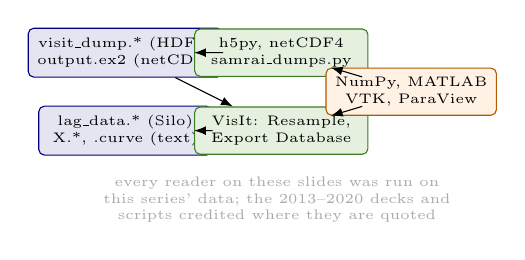
\begin{tikzpicture}[scale=0.55, every node/.style={font=\tiny}]
  \node[draw=NavyBlue,fill=NavyBlue!10,rounded corners=2pt,minimum width=2.2cm,minimum height=0.5cm,align=center] (a) at (0,0.9) {\code{visit\_dump.*} (HDF5)\\\code{output.ex2} (netCDF)};
  \node[draw=NavyBlue,fill=NavyBlue!10,rounded corners=2pt,minimum width=2.2cm,minimum height=0.5cm,align=center] (b) at (0,-0.9) {\code{lag\_data.*} (Silo)\\\code{X.*}, \code{.curve} (text)};
  \node[draw=OliveGreen,fill=OliveGreen!10,rounded corners=2pt,minimum width=2.2cm,minimum height=0.5cm,align=center] (p) at (3.6,0.9) {h5py, netCDF4\\\code{samrai\_dumps.py}};
  \node[draw=OliveGreen,fill=OliveGreen!10,rounded corners=2pt,minimum width=2.2cm,minimum height=0.5cm,align=center] (v) at (3.6,-0.9) {VisIt: Resample,\\Export Database};
  \node[draw=orange!70!black,fill=orange!10,rounded corners=2pt,minimum width=2.0cm,minimum height=0.5cm,align=center] (f) at (6.6,0) {NumPy, MATLAB\\VTK, ParaView};
  \draw[-{Latex[length=1.5mm]}] (a) -- (p); \draw[-{Latex[length=1.5mm]}] (b) -- (v); \draw[-{Latex[length=1.5mm]}] (a) -- (v);
  \draw[-{Latex[length=1.5mm]}] (p) -- (f); \draw[-{Latex[length=1.5mm]}] (v) -- (f);
  \node[text=DarkGray,align=center,text width=5.3cm] at (3.5,-2.5) {every reader on these slides was run on this series' data; the 2013--2020 decks and scripts credited where they are quoted};
\end{tikzpicture}}
\end{frame}

% 2
\begin{frame}{Learning goals}
\label{fr:goals}
\footnotesize By the end of this chapter you should be able to:
\begin{enumerate}
  \item name every file an IBAMR run writes, its container (HDF5, netCDF, Silo, text) and what reads it (VisIt, Python, MATLAB), and set the input keys that control them;
  \item read the fluid dumps straight into NumPy (\code{samrai\_dumps.py}) or MATLAB (\code{samrai\_dumps.m}), put the adaptive patches on a uniform grid, and check the result against VisIt;
  \item do the same through VisIt, with the Resample operator and \gui{Export Database} (the 2017--2018 recipe), scripted for a series of frames (\code{resample\_export.py}), and know the five things that silently give an empty file in 3.5;
  \item read the exported VTK, the ExodusII file of an IBFE run, the Silo points and the HDF5 state dumps with the readers of \code{examples/analysis}, in Python and in MATLAB/Octave;
  \item compute a quantity VisIt does not give you directly, the flow rate across a line against time, from the dumps (the 2020 lecture's \code{flappy\_ends.m}, redone on IB/02 and IB/11);
  \item bring other programs' fields into VisIt (PIV components to VTK, COMSOL's VTU) and know where ParaView, Tecplot and the LCS tools fit.
\end{enumerate}
\begin{punchbox}
\scriptsize Everything shown was run: the readers on IB/13, IB/02, IB/11, IBFE/01, IBFE/10 and an upstream run, with Python 3.12 (h5py 3.10, netCDF4 1.6, vtk 9.1, meshio 5.3) and Octave 8.4 (netcdf 1.0.17) in WSL; MATLAB itself was not available, so the \code{.m} files were checked in Octave where Octave has the function (netCDF yes, \code{h5read} no).
\end{punchbox}
\end{frame}

% 3
\begin{frame}{Where this chapter comes from}
\label{fr:sources}
\scriptsize
\begin{itemize}
  \item \al{``Taking a 2D slice from 3D IBAMR with Visit'' (2017, 17 slides) and ``6 -- Resampling AMR grids to Uniform Grid, exporting to .vtk, and recording in Python'' (2018, 21 slides):} the Resample operator, the plane of one sample, \gui{Export Database} to VTK, the \code{2D\_Slicer.py} recording with its time loop, Nick's MATLAB reader, the \code{mopenpiv} reader, the ``cut off the edges'' warning, the KillDevil commands. Quoted and redone in 3.5 (slides \ref{fr:resample}--\ref{fr:plane}).
  \item \al{``Converting IBAMR output to Matlab and analyzing it'' (MATH 769, 23 April 2013, 12 slides) and ``5 -- Reading forces and converting IBAMR output to Matlab and analyzing it'' (2020, 24 slides):} Eric Tytell's \code{importsamrai.m} and its \code{V} structure, the \code{OUTPUT\_DIV\_U} workaround, \code{flappy\_ends.m} and \code{vol\_flow\_rate.m}, \code{pcolor\_frames.m}; the Lagrangian half is chapter 11, the Eulerian half is here (slides \ref{fr:importsamrai}, \ref{fr:flow}--\ref{fr:frames}).
  \item \al{Christopher Strickland's 2017 scripts and README} (``IBAMR $\to$ VTK $\to$ NumPy''): \code{read\_IBAMR3d\_py27.py} and \code{read\_vtk\_data.py}; \al{Nick Battista's 2017 MATLAB readers} \code{read\_Structured\_Vector\_Field\_Data\_From\_vtk.m} and \code{Convert\_vtk2LCS.m}; the lab's 2017 Read Me notes on batch processing (Lindsay Waldrop), LCS options, Dabiri's LCS code and Arvind's circulation script; the 2017 ``Read Me and To Do'' whose item ``overview of translating one file type to another (.visit, .m, .py, .txt, .vtk, etc)'' was the one-slide stub this chapter fills.
  \item \al{The 2019 ``6. Analyze PIV Data'' document} (DaVis batch processing; the lost \code{toVTK.py}) and \al{the 2020 COMSOL lecture's slides 12--14} (export as VTU, open in VisIt).
  \item \al{New here:} the file formats read from the files themselves (\code{h5py}, \code{ncdump}); \code{samrai\_dumps.py/.m}, \code{read\_exodus.py/.m}, \code{read\_vtk\_legacy.py/.m}, \code{hier\_data\_h5.py}, \code{resample\_export.py}, \code{flow\_rate.py}, \code{piv\_to\_vtk.py} in \code{examples/analysis}, each tested; the comparison of the Python route with VisIt's; what VisIt 3.5 does wrong headless.
\end{itemize}
\end{frame}

% 4
\begin{frame}{The map: what a run writes, and what reads it (1)}
\label{fr:map}
\scriptsize
\renewcommand{\arraystretch}{0.95}
\begin{tabular}{@{}L{0.24\textwidth}L{0.17\textwidth}L{0.18\textwidth}L{0.31\textwidth}@{}}
\toprule
file & written by & container & readers \\
\midrule
\code{viz\_IB2d/dumps.visit}, \code{visit\_dump.NNNNN/} & SAMRAI's VisIt writer, every \code{viz\_dump\_interval} & HDF5 (\code{summary.samrai} + one \code{processor\_cluster} file per rank) & VisIt (SAMRAI plugin); Python \code{h5py} via \code{samrai\_dumps.py}; MATLAB \code{h5read} via \code{samrai\_dumps.m}; not ParaView's own readers \\
\code{viz\_IB2d/}\allowbreak\code{lag\_data.visit}, \code{lag\_data.}\allowbreak\code{cycle\_NNNNNN/} & \code{LSiloDataWriter} (chapter 28) & Silo, PDB driver (not HDF5) & VisIt; export from VisIt as VTK; the \code{X.*} files hold the same positions \\
\code{viz\_IB2d/output.ex2} (one per part) & libMesh's \code{ExodusII\_IO} (IBFE) & ExodusII = netCDF-4/HDF5 & VisIt, ParaView; Python \code{netCDF4} via \code{read\_exodus.py}; MATLAB \code{ncread} via \code{read\_exodus.m} \\
\code{hier\_data\_IB2d/X.NNNNN}, \code{F.NNNNN} & the examples' \code{output\_data} (chapter 11) & PETSc ASCII text & \code{hier\_data.py}, \code{read\_hier\_data.m} \\
\bottomrule
\end{tabular}
\end{frame}

% 4b
\begin{frame}{The map (2): curves, VTK, restart files, and the keys}
\label{fr:map2}
\scriptsize
\renewcommand{\arraystretch}{0.95}
\begin{tabular}{@{}L{0.24\textwidth}L{0.17\textwidth}L{0.18\textwidth}L{0.31\textwidth}@{}}
\toprule
file & written by & container & readers \\
\midrule
\code{hier\_data\_IB2d/}\allowbreak\code{hier\_data.NNNNN.}\allowbreak\code{samrai.PPPPP} & SAMRAI's HDF5 database (upstream ex1, the IBFE and complex-fluid examples) & HDF5 & \code{hier\_data\_h5.py} \\
\code{*.curve} & VisIt (queries over time, picks, lineouts) & text & \code{importdata}, \code{numpy} (chapter 28) \\
\code{*.vtk}, \code{*.vtr} & VisIt's \gui{Export Database}; IB2d's own output & VTK legacy or XML & VisIt, ParaView; \code{read\_vtk\_legacy.py/.m}, the \code{vtk} module, \code{pyvista} \\
\code{restart\_IB2d/} & SAMRAI + \code{writeFEData}\allowbreak\code{ToRestartFile} & HDF5 + libMesh xda & the program only \\
\bottomrule
\end{tabular}

\vspace{1mm}
\footnotesize The input keys: \code{viz\_writer}, \code{viz\_dump\_interval}, \code{viz\_dump\_dirname}, \code{data\_dump\_interval}, \code{data\_dump\_dirname}, \code{restart\_dump\_interval} in \code{Main} (chapter 7); \code{output\_U}, \code{output\_P}, \code{output\_Omega}, \code{output\_Div\_U} in the integrator block choose the fluid fields.
\end{frame}

% 5
\begin{frame}[fragile]{The fluid dumps on disk}
\label{fr:disk}
\footnotesize
\begin{columns}[T]
\column{0.5\textwidth}
\begin{lstlisting}[style=tiny]
viz_IB2d/                            # IB/13 human, 4 ranks, 102 frames
  dumps.visit                        # visit_dump.00000/summary.samrai ...
  visit_dump.19096/                  # frame 56: the time step number
    summary.samrai                   # 20 kB: the hierarchy and the extents
    processor_cluster.00000.samrai   # 115 kB: rank 0's patches and fields
    processor_cluster.00001.samrai   # 114 kB
    processor_cluster.00002.samrai   #  99 kB
    processor_cluster.00003.samrai   #  99 kB
\end{lstlisting}
\begin{lstlisting}[style=shell]
$ file visit_dump.19096/summary.samrai
Hierarchical Data Format (version 5) data
$ h5ls -r visit_dump.19096/summary.samrai | head   # hdf5-tools
$ python3 -c "import h5py; f = h5py.File('summary.samrai'); f.visit(print)"
\end{lstlisting}
\column{0.48\textwidth}
\scriptsize
\begin{itemize}
  \item A frame is a folder named by the time step, holding one HDF5 file per MPI rank with the data and one summary file with the layout; \code{dumps.visit} lists the summary files in order (chapter 26). The same for 3D (\code{viz\_IB3d/}).
  \item They are HDF5 files whatever their extension: \code{h5ls}, \code{h5dump} (apt \code{hdf5-tools}) and \code{h5py} open them; nothing in them is private to VisIt.
  \item The values are single precision (\code{float32}) and nodal for \code{U}, \code{P}, \code{Omega} (IBAMR 0.12 on), cell-centred for \code{Div U}: these are VisIt's copies, not the solver's arrays. The solver's own double-precision state is the \code{hier\_data.*.samrai.*} dump of slide \ref{fr:hierh5}, when a program writes it.
  \item Sizes: the human carotid run's 102 frames take 49 MB; the 512$^2$ channel's 51 frames 38 MB; a 3D run grows fast, which is why one dumps every few hundred steps and not every step (chapter 7's interval table).
\end{itemize}
\end{columns}
\end{frame}

% 6
\begin{frame}[fragile]{Inside \code{summary.samrai}}
\label{fr:summary}
\footnotesize
\begin{columns}[T]
\column{0.54\textwidth}
\begin{lstlisting}[style=tiny]
BASIC_INFO/
  number_dimensions_of_problem  [2]
  var_names             [b'U', b'P', b'Omega', b'Div U']
  var_cell_centered     [0, 0, 0, 1]        # 0 = nodal
  var_number_components [2, 1, 1, 1]        # U has U.00, U.01
  var_number_ghosts     [[0,0,0], ...]
  number_levels         [2]
  number_patches_at_level [4, 6]            # 10 patches in all
  number_processors     [4]   number_file_clusters [4]
  dx                    [[0.125, 0.125, 0], [0.03125, 0.03125, 0]]
  XLO                   [0, 0, 0]
  ratios_to_coarser_levels [[-1,-1,0], [4,4,0]]
  time [0.9548]   time_step_number [19096]   grid_type [b'CARTESIAN']
extents/
  patch_extents  (10,) lower, upper, xlo, xup     # per patch
     e.g. lower (0,0) upper (12,23) xlo (0,0) xup (1.625,3.0)
  patch_map      (10,) processor, file cluster, level, patch number
  Omega-Extents  (10,) data_is_defined, min, max, ...  # per patch, per variable (two more flags)
\end{lstlisting}
\column{0.44\textwidth}
\scriptsize
\begin{itemize}
  \item Everything the reader needs: the variables and their centering, the levels and their spacings, the refinement ratios, and for every patch its index box (\code{lower}, \code{upper}, inclusive, in the cells of its own level), its physical box, and which rank's file holds it.
  \item The level-0 patches tile the domain: their \code{upper} maxima plus one give the coarse cell count ($50 \times 24$ here), and the ratios the finest ($200 \times 96$).
  \item The per-variable extents are the file's own minimum and maximum: a check for any reader (\code{Omega} runs from $-3272.4$ to $3474.7$ at this frame; the reader reproduces both).
  \item The 2013 lecture's \code{OUTPUT\_DIV\_U = FALSE} workaround (``the space in the name'') is not needed: \code{Div U} is an ordinary dataset name to HDF5.
\end{itemize}
\end{columns}
\end{frame}

% 7
\begin{frame}[fragile]{Inside the \code{processor\_cluster} files}
\label{fr:cluster}
\footnotesize
\begin{columns}[T]
\column{0.5\textwidth}
\begin{lstlisting}[style=tiny]
processor.00000/
  level.00000/
    patch.00000/
      Div U   (312,)  >f4      # 13 x 24 cells
      Omega   (350,)  >f4      # 14 x 25 nodes
      P       (350,)  >f4
      U.00    (350,)  >f4      # the x component
      U.01    (350,)  >f4
  level.00001/
    patch.00000/   Div U (3120,)  Omega (3233,) ...
    patch.00001/   Div U (480,)   Omega (549,)  ...
\end{lstlisting}
\begin{lstlisting}[style=pytiny]
a = g["Omega"][()]                  # flat, x fastest (SAMRAI's order)
ncell = upper - lower + 1           # (13, 24)
A = a.reshape((ncell + 1)[::-1])    # nodal: (25, 14) = [y, x]
\end{lstlisting}
\column{0.48\textwidth}
\scriptsize
\begin{itemize}
  \item Each rank's file holds only its own patches, grouped by level and patch number; the patch's index box is in the summary file (slide \ref{fr:summary}); a cell-centred variable has $n_x n_y$ values, a nodal one $(n_x + 1)(n_y + 1)$ ($13 \times 24 = 312$ and $14 \times 25 = 350$ for patch 0).
  \item The arrays are flat with $x$ varying fastest, so \code{reshape((ny, nx))} gives an array indexed \code{[y, x]}, the orientation \code{pcolormesh} and MATLAB's \code{meshgrid} expect.
  \item A vector is stored as components \code{U.00}, \code{U.01} (\code{U.02} in 3D); VisIt reassembles \code{U} from them, a reader does the same.
  \item \code{>f4}: big-endian single precision (HDF5 converts on reading); the values are the nodal interpolants VisIt plots, not the staggered-grid velocities of the solver.
  \item Ghost cells: \code{var\_number\_ghosts} is zero for these files, so the arrays cover exactly the patch; the \code{hier\_data} HDF5 dumps of slide \ref{fr:hierh5} record a ghost width per patch (\code{d\_ghosts}), zero in the dumps read there.
\end{itemize}
\end{columns}
\end{frame}

% 8
\begin{frame}[fragile]{\code{samrai\_dumps.py}: the reader}
\label{fr:reader}
\footnotesize
\begin{columns}[T]
\column{0.52\textwidth}
\begin{lstlisting}[style=pytiny]
import samrai_dumps as sd
d = sd.Dump("viz_IB2d/visit_dump.19096")      # one frame
d.time, d.levels, d.patches_per_level         # 0.9548, 2, [4, 6]
d.variables                                   # ['U', 'P', 'Omega', 'Div U']
x, y, omega = d.uniform("Omega")              # finest grid: x (201,), y (97,), omega (97, 201)
x, y, (u, v) = d.uniform("U")                 # a vector: one array per component
x, y, divu = d.uniform("Div U")               # cell-centred: x (200,), y (96,)
d.patch_extent_values("Omega")                # ([-3272.36], [3474.73]) from the summary
for step, t, folder in sd.frames("viz_IB2d"): # the series from dumps.visit
    d = sd.Dump(folder); ...; d.close()
\end{lstlisting}
\begin{lstlisting}[style=tiny]
$ python3 samrai_dumps.py viz_IB2d/visit_dump.19096 Omega
time 0.9548 step 19096  levels 2  patches [4, 6]  finest cells [200, 96]  dx [0.03125, 0.03125]
  U      nodal  components 2  file extents ([-30.02, -65.59], [110.97, 52.80])
  P      nodal  components 1  file extents ([-1748.2], [14797.5])
  Omega  nodal  components 1  file extents ([-3272.36], [3474.73])
  Div U  cell   components 1  file extents ([-0.1426], [0.3614])
  Omega[0] on the uniform grid: shape (97, 201), min -3272.36 max 3474.73, NaN 0
\end{lstlisting}
\column{0.46\textwidth}
\scriptsize
\begin{itemize}
  \item \code{examples/analysis/samrai\_dumps.py}: 220 lines, \code{numpy} and \code{h5py} only. \code{Dump} reads the summary, opens the rank files as needed, \code{patch\_data(patch, var)} gives one patch's arrays, \code{uniform(var, level)} the whole domain on one level's grid, \code{frames(viz\_dir)} the list from \code{dumps.visit} with the times.
  \item \code{uniform} paints the levels coarse to fine: a coarse patch is interpolated onto the fine nodes (bilinear) or repeated per cell (cell-centred data), and a finer patch overwrites it wherever it exists. Nodal data come back on the nodes of the finest level ($N + 1$ per direction), cell data on the centres ($N$).
  \item The arrays are \code{[y, x]} (\code{[z, y, x]} in 3D, filled the same way: trilinear for nodal data, repeated for cell data); \code{nan} marks nothing here, because the level-0 patches cover the box.
  \item \code{line\_flux(x, y, u, x0, ylo, yhi)} integrates a field across a vertical line (slide \ref{fr:flow}).
\end{itemize}
\end{columns}
\end{frame}

% 9
\begin{frame}{From patches to a uniform grid}
\label{fr:uniform}
\begin{columns}[T]
\column{0.5\textwidth}\centering
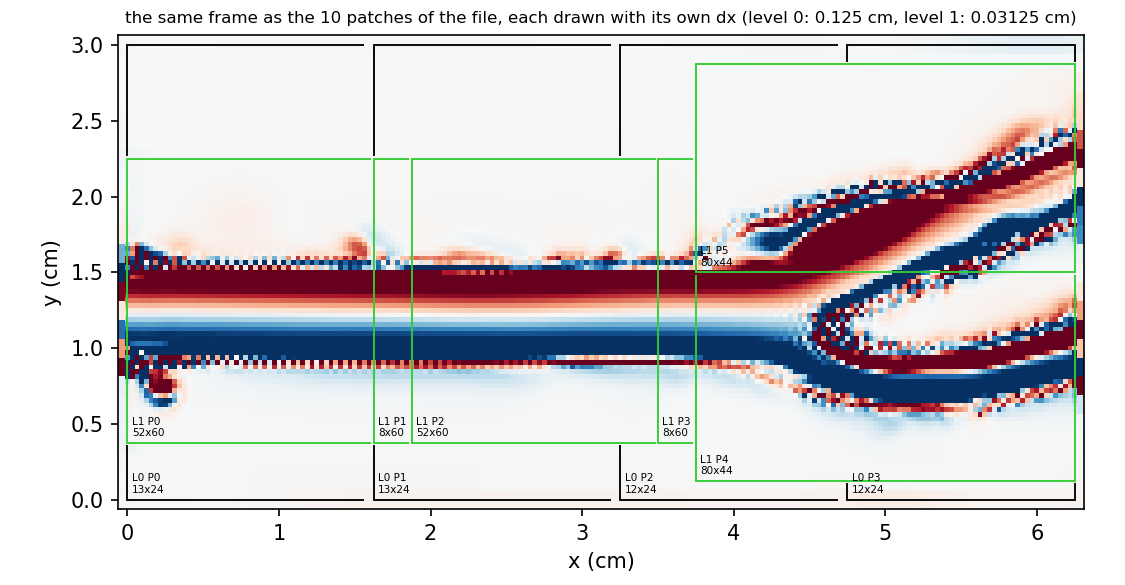
\includegraphics[width=0.9\textwidth]{ch33-py-patches.png}\\
\scriptsize the ten patches of frame 56 as the file holds them, each drawn with its own spacing (level 0 black, level 1 green)
\column{0.5\textwidth}\centering
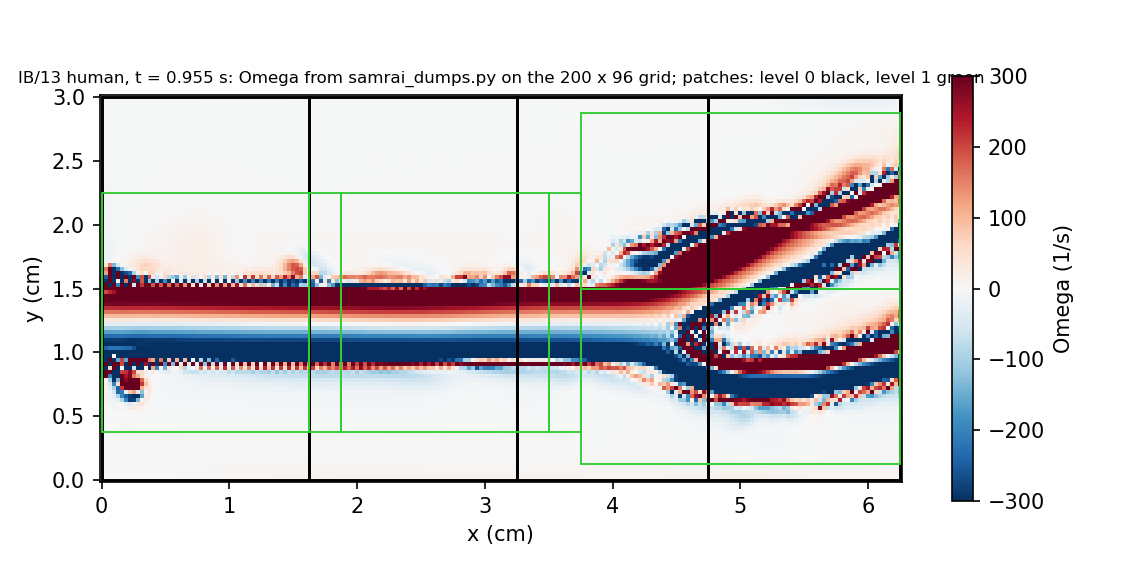
\includegraphics[width=0.9\textwidth]{ch33-py-omega.png}\\
\scriptsize \code{d.uniform("Omega")}: the same frame on the $200 \times 96$ grid of level 1, the patch boxes drawn over it
\end{columns}
\footnotesize
\begin{itemize}
  \item The AMR hierarchy is a set of rectangles; where a level-1 patch exists its nodes are the fine grid's nodes, and elsewhere the level-0 values are interpolated to them: nothing is invented, the picture is smooth across the patch edges because the coarse data are linear across them.
  \item A uniform array is what every analysis wants: a flux across a line, a time average at a point, a Fourier transform in $x$, a comparison with PIV on its regular grid, a MATLAB \code{pcolor}. The price is the memory of the finest grid everywhere ($200 \times 96$ here; $512^2$ for the channel; a 3D run's finest grid can be larger than the machine wants, so take a plane with \code{uniform(..., level=k)} on a coarser level or VisIt's Resample with a box).
\end{itemize}
\end{frame}

% 10
\begin{frame}{Checked against VisIt}
\label{fr:check}
\footnotesize
\begin{itemize}
  \item VisIt's \gui{Resample} operator on the same frame, with the sample points put exactly on the fine nodes ($201 \times 97$ over $[0, 6.25] \times [0, 3]$), exported as VTK and read back: the two \code{Omega} arrays agree to $0.012$ at worst on a range of $6747$ ($1.8 \times 10^{-6}$ relative, rms $3 \times 10^{-4}$); $18$ of the $19\,497$ nodes differ by more than $10^{-6}$ of $\max|\Omega|$ (five by more than $10^{-6}$ of the range), most of them within four cells of the inlet boundary $x = 0$, where VisIt's interpolation is its own. The reader reproduces the file's extents exactly; VisIt's resample is within $2 \times 10^{-3}$ of them.
  \item \code{U} the same way (VisIt's export of the vector: components agree to $6 \times 10^{-5}$, single precision).
  \item So the Python route and the VisIt route are the same numbers; choose by convenience: Python when the analysis is a loop over frames or a quantity VisIt has no query for, VisIt when a picture or one of its queries is enough (chapter 29).
  \item Chapter 16's convergence study, chapter 24's exercise (the average of $T$) and chapter 9b's pump measures (the kinetic energy of the flow) are the kind of thing the reader is for.
\end{itemize}
\begin{punchbox}
\scriptsize The upstream \code{ex1} that the examples' \code{output\_data} descends from also wrote the Eulerian fields as HDF5 (\code{hier\_data.NNNNN.samrai.PPPPP}, slide \ref{fr:hierh5}); this series' examples dropped that, because the VisIt dumps already hold the fields and this reader opens them.
\end{punchbox}
\end{frame}

% 11
\begin{frame}[fragile]{The MATLAB version, and Tytell's \code{importsamrai.m} (2013)}
\label{fr:importsamrai}
\footnotesize
\begin{columns}[T]
\column{0.5\textwidth}
\begin{lstlisting}[style=mtiny]
% examples/analysis/samrai_dumps.m (MATLAB, h5read)
d = samrai_dumps('viz_IB2d/visit_dump.19096');          % the layout
d = samrai_dumps('viz_IB2d/visit_dump.19096', 'Omega'); % + d.x, d.y, d.data (ny x nx)
pcolor(d.x, d.y, d.data); shading flat; axis equal
d = samrai_dumps(folder, 'U');                          % d.data{1}, d.data{2}
\end{lstlisting}
\begin{lstlisting}[style=mtiny]
% the 2013 / 2020 lecture (E. Tytell's toolbox, matlab-tytell/CFD, after install_here.m)
[x,y,Vinterp,V] = importsamrai(pathname,'interpolaten',[GridSizex GridSizey])
% V(k).level_number, .xlo, .xup, .rows, .cols: one element per patch
% V(k).U_0, .U_1, .P, .F0, .F1, .Omega: the fields of that patch
% Vinterp: the same interpolated to the GridSizex x GridSizey grid
\end{lstlisting}
\column{0.48\textwidth}
\scriptsize
\begin{itemize}
  \item \code{samrai\_dumps.m} mirrors the Python reader line by line with \code{h5read} (MATLAB's HDF5 reader; it returns the arrays transposed, which the code undoes), \code{kron} for cell data and \code{interp2} for nodal data. It was written against the Python output and not run: Octave 8 has no \code{h5read} and MATLAB was not at hand. 2D only.
  \item The 2013 lecture used Eric Tytell's \code{importsamrai.m}: ``imports samrai data from files in the directory pathname. Files should be named \code{summary.samrai} and \code{processor\_clusterXXXXX.samrai}''; its output \code{V} is ``a structure containing one element for each grid region'' with \code{level\_number} ``from 1 (coarsest) usually to 4 (finest)'', \code{xlo}, \code{xup}, \code{rows}, \code{cols} and the fields, and \code{Vinterp} the interpolated data. The same idea; its fields are the old names (\code{U\_0}, \code{F0}) and it needed \code{OUTPUT\_DIV\_U = FALSE} ``due to the space in the name''. The toolbox is third-party (link in chapter 11) and not shipped.
  \item \code{Forceread.m} and \code{positionread.m} of the same lecture are chapter 11's \code{read\_hier\_data.m}.
\end{itemize}
\end{columns}
\end{frame}

% 12
\begin{frame}{VisIt's route: the Resample operator (2017--2018)}
\label{fr:resample}
\begin{columns}[T]
\column{0.36\textwidth}\centering
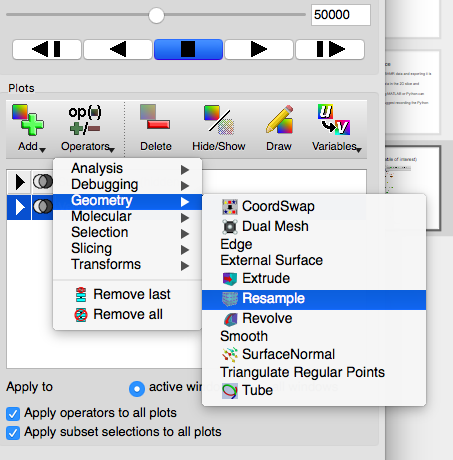
\includegraphics[width=\textwidth]{ch33-d18-resample-menu.png}\\
\scriptsize \gui{Operators $\to$ Geometry $\to$ Resample} (2017/2018 decks, VisIt 2.7.1)
\column{0.36\textwidth}\centering
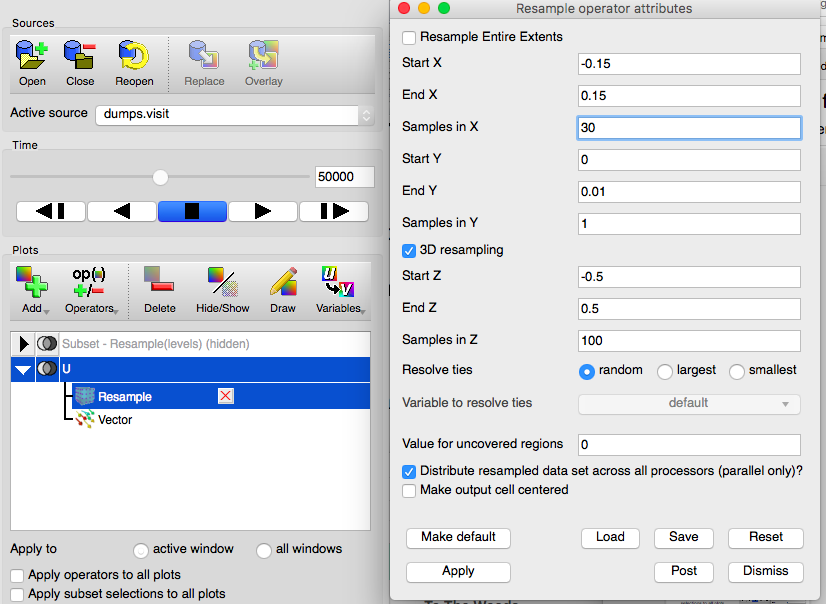
\includegraphics[width=\textwidth]{ch33-d18-resample-attr.png}\\
\scriptsize the attributes: a plane of $30 \times 1 \times 100$ samples at $y \in [0, 0.01]$
\column{0.26\textwidth}
\scriptsize
\begin{enumerate}
  \item Open \code{dumps.visit}, plot \code{U} (or the variable of interest).
  \item ``Unclick apply operators to all plots. Unclick apply subset selections to all plots.''
  \item Highlight the plot, \gui{Operators $\to$ Geometry $\to$ Resample}; double-click it.
  \item ``Unclick resample entire extents''; set the samples and the start/end of each direction; \gui{Apply}.
\end{enumerate}
\end{columns}
\sourcecredit{Windows: ``6 -- Resampling AMR grids'' (2018; the same images as the 2017 deck), VisIt 2.7.1 on a Mac.}
\end{frame}

\begin{frame}{What the Resample operator does}
\label{fr:resample2}
\footnotesize
\begin{itemize}
  \item ``The main issue with taking a 2D slice from 3D IBAMR data and exporting it is that it is on an adaptive grid. We can handle this in Visit by resampling the data in the 2D slice and exporting it to vtk'' (2017). Resample puts the plotted variable on a regular grid of \code{samplesX} $\times$ \code{samplesY} $\times$ \code{samplesZ} points between the start and end values (\code{useExtents = 1} takes the whole domain); \code{defaultValue} fills points no patch covers; \code{distributedResample} shares the work among a parallel engine's processes (on, VisIt 3.5.0 exported each state in pieces written into one file, so \code{resample\_export.py} turns it off; chapter 31); \code{cellCenteredOutput} makes cells instead of nodes.
  \item The 3.5 window has the same fields (\gui{Resample Entire Extents}, \gui{Start X} \ldots, \gui{Samples in Z}, \gui{3D resampling}, \gui{Resolve ties}, \gui{Value for uncovered regions}, \gui{Distribute resampled data set}, \gui{Make output cell centered}).
\end{itemize}
\end{frame}

% 13
\begin{frame}{Export the resampled data: \gui{File $\to$ Export Database}}
\label{fr:export}
\begin{columns}[T]
\column{0.34\textwidth}\centering
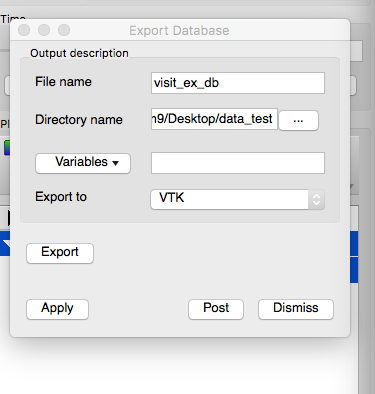
\includegraphics[width=0.9\textwidth]{ch33-d18-export.png}\\
\scriptsize the Export window (2018): name, directory, variables, \gui{Export to: VTK}
\column{0.64\textwidth}
\footnotesize
\begin{itemize}
  \item ``Highlight Resample. Go to File $\to$ Export database. Choose your file name and directory. Export to VTK. If you choose no variables, it will just export U. Click export.'' (2018). The export writes the active plot's data \emph{after its operators}: with Resample on it, a regular grid (VTK \code{RECTILINEAR\_GRID}); the variables added in the window come along, resampled too.
  \item ``You can also export .ex2 files to vtk'' (chapter 28 did it: the mesh and \code{dX}).
  \item The warning that still holds: ``When you resample, if the grid is very coarse in places (especially the edges), those values may be set to zero. The solution when doing your analysis is to cut off the edges of the domain.'' (\code{defaultValue} is what you see there.)
  \item The result ``has the vector U = (Ux, Uy, Uz) in the (x, y, z) plane''; the 2017 deck's example was a plane of $30 \times 100$ points through a 3D run, ``use only U = (Ux, Uz) in the (x, z) plane''.
\end{itemize}
\end{columns}
\sourcecredit{Window: ``6 -- Resampling AMR grids'' (2018; the same image as the 2017 deck), VisIt 2.7.1 on a Mac.}
\end{frame}

% 14
\begin{frame}{Five ways VisIt 3.5 gives you an empty export, headless (1)}
\label{fr:empty}
\footnotesize All found while scripting the recipe on this series' runs (\code{wsl/final/ch33\_*.sh}); none shows an error.
\begin{enumerate}
  \item \al{The file name and directory are ignored:} every export writes \code{.vtk} (no name) into the \emph{current directory} of the VisIt process, and \gui{Export all time states} overwrites it state after state. Rename the file after each export (\code{resample\_export.py} does); the GUI on a desktop may behave, chapter 28 reported the same for the Exodus export.
  \item \al{A SAMRAI database reports zero extents} in its metadata (\code{GetMetaData(db).GetMeshes(0).minSpatialExtents} is all zeros), so a resample box built from them is a point and the file holds zeros: ask the drawn plot instead (\code{Query("SpatialExtents")}), or type the box.
  \item \al{A plane of zero thickness exports zeros:} \code{samplesY = 1} with \code{startY = endY} resamples nothing; the 2017 deck's \code{startY = 0, endY = 0.01} was this fix (a slab one per cent of the axis thick works; two samples work too).
\end{enumerate}
\end{frame}

\begin{frame}{Five ways VisIt 3.5 gives you an empty export (2), and a reader that cannot read them}
\label{fr:empty2}
\footnotesize
\begin{enumerate}
\setcounter{enumi}{3}
  \item \al{In one session, a Vector plot exported a broken grid} (coordinate lists of one entry) and a Pseudocolor of the automatic \code{U\_magnitude} expression exported \code{U} as zeros; a later re-test of both exported correctly (VisIt only warns that the Vector plot ``yielded no data''), so treat these two as possible, not certain. Plot a Pseudocolor of a scalar (\code{U[0]} as an expression) and add \code{U} in the variable list: that route exported correctly every time.
  \item \al{An export without Resample} (the AMR mesh itself) creates a named directory and a \code{.visit} list, but headless 3.5.0 writes every patch file as \code{<cwd>/.vtk}, each overwriting the last, and the list points at \code{<dir>/.vtk}: nothing can read the result (reproduced twice). Resample first, or move each patch file yourself.
\end{enumerate}
\begin{punchbox}
\scriptsize \code{meshio} 5.3 cannot read VisIt's legacy VTK files (their \code{FIELD} block has a string entry, \code{MeshName}: ``\code{'string'}'') and does not know \code{.vtr}; the \code{vtk} module and \code{read\_vtk\_legacy.py} read them, \code{pyvista} reads \code{.vtr}.
\end{punchbox}
\end{frame}

% 15
\begin{frame}[fragile]{\code{resample\_export.py}: the recipe scripted for a series of frames}
\label{fr:script}
\footnotesize
\begin{columns}[T]
\column{0.64\textwidth}
\begin{lstlisting}[style=tiny]
$ visit -nowin -cli -s resample_export.py -- viz_IB2d/dumps.visit U out nx=201 ny=97 states=56
state 56  t = 0.9548  ->  out/U_0056.vtk
   (ok; plot U_c0 -- Min = -30.02 ... Max = 110.97 ...)
$ visit -nowin -cli -s resample_export.py -- viz_IB3d/dumps.visit U plane \
      nx=141 ny=1 nz=101 x0=-4 x1=10 y0=0 z0=-5 z1=5 states=all
\end{lstlisting}
\begin{lstlisting}[style=pytiny]
OpenDatabase(db); DeleteAllPlots()                  # the automatic 'levels' Subset plot goes
DefineScalarExpression("U_c0", "U[0]"); AddPlot("Pseudocolor", "U_c0"); DrawPlots()
Query("SpatialExtents"); ext = GetQueryOutputValue()  # the box (the metadata's is zero)
AddOperator("Resample"); r = ResampleAttributes(); r.useExtents = 0
r.startX, r.endX, r.samplesX = x0, x1, nx; ...; r.is3D = 1; r.defaultValue = 0
SetOperatorOptions(r)
e = ExportDBAttributes(); e.db_type = "VTK"; e.db_type_fullname = "VTK_1.0"
e.dirname = out; e.variables = ("U",); opts = GetExportOptions("VTK")
for s in states:
    SetTimeSliderState(s); DrawPlots(); e.filename = "U_%04d" % s
    ExportDatabase(e, opts)                          # writes <cwd>/.vtk ...
    os.replace(".vtk", os.path.join(out, "U_%04d.vtk" % s))   # ... so rename it
\end{lstlisting}
\column{0.34\textwidth}
\scriptsize
\begin{itemize}
  \item Left: how the script is called, and what it prints per state (the plot's \gui{MinMax}, so that an empty export shows up at once); below it, the lines that matter, from the file in \code{examples/analysis}. The next slide says what the script is and where it comes from.
\end{itemize}
\end{columns}
\end{frame}

\begin{frame}{\code{resample\_export.py}: what it is, and its ancestors (2017)}
\label{fr:script2}
\footnotesize
\begin{itemize}
  \item \code{examples/analysis/resample\_export.py} runs inside VisIt's Python (\code{visit -nowin -cli -s}, chapter 32): the database, the variable, the output folder, the samples, the box, the states, legacy ASCII or binary output. It prints the plot's \gui{MinMax} at each state as a check that the data are there.
  \item Its ancestors: the 2017 \code{2D\_Slicer.py} (the recording of the GUI steps with \code{TimeSliderNextState()} in a \code{while} loop, \code{ExportDBAtts.filename = "visit\_ex\_db\_\%s" \% k}) and Christopher Strickland's \code{read\_IBAMR3d\_py27.py} (2017: Python 2.7, \code{sys.path.append} to VisIt 2.11's \code{site-packages}, \code{LaunchNowin()}, $11^3$ samples over the full extents by default, files \code{vtk3d/<run>/IBAMR\_db\_NNN.vtk}, and a note on fixing \code{frontend.py} on Windows). VisIt 3 embeds Python 3 and none of the path tricks is needed.
  \item The recording itself (\gui{Controls $\to$ Command}, Record) is chapter 32; the 2018 deck's slides 15--21 (KillDevil modules, \code{visit -nowin -cli -s script.py}) are chapters 31--32.
\end{itemize}
\end{frame}

% 16
\begin{frame}{A 2D plane out of a 3D run}
\label{fr:plane}
\begin{columns}[T]
\column{0.3\textwidth}\centering
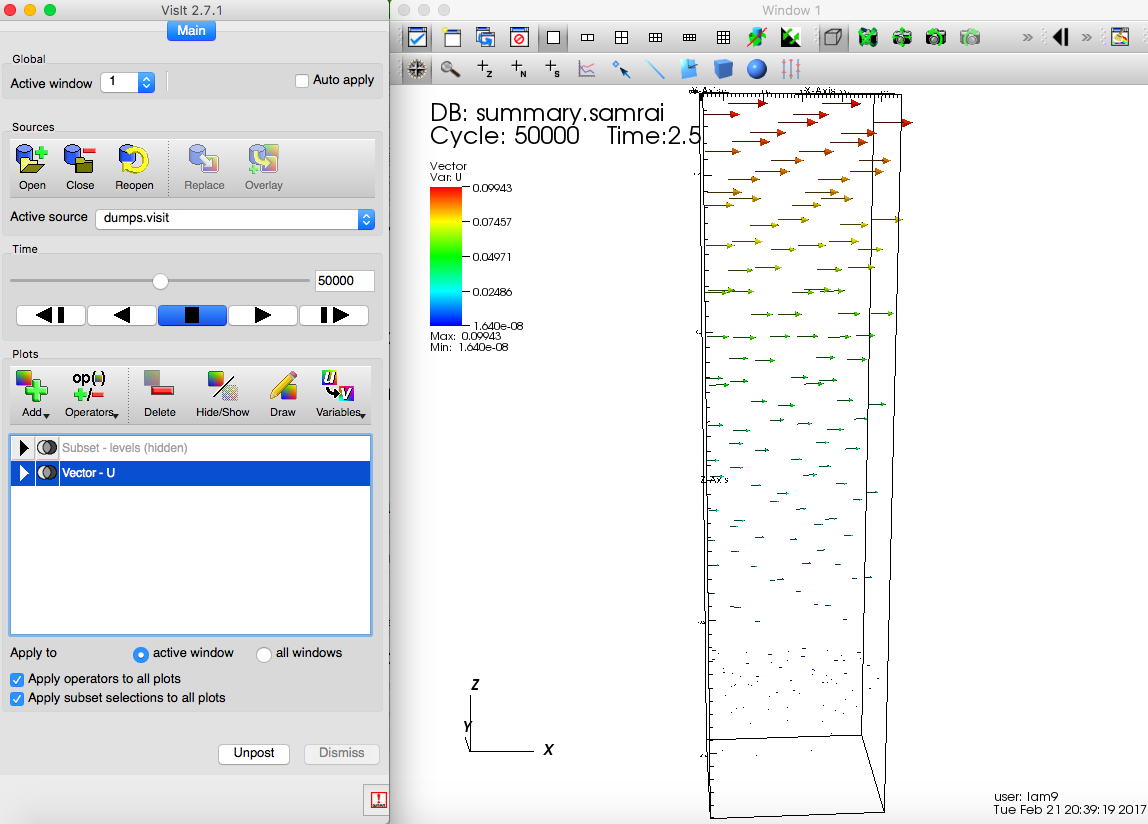
\includegraphics[width=0.9\textwidth]{ch33-d18-plane-vectors.png}\\
\scriptsize 2017: the resampled plane's $30 \times 100$ vectors in the 3D view (a tower of coral, \code{sample\_viz\_IB3d})
\column{0.3\textwidth}\centering
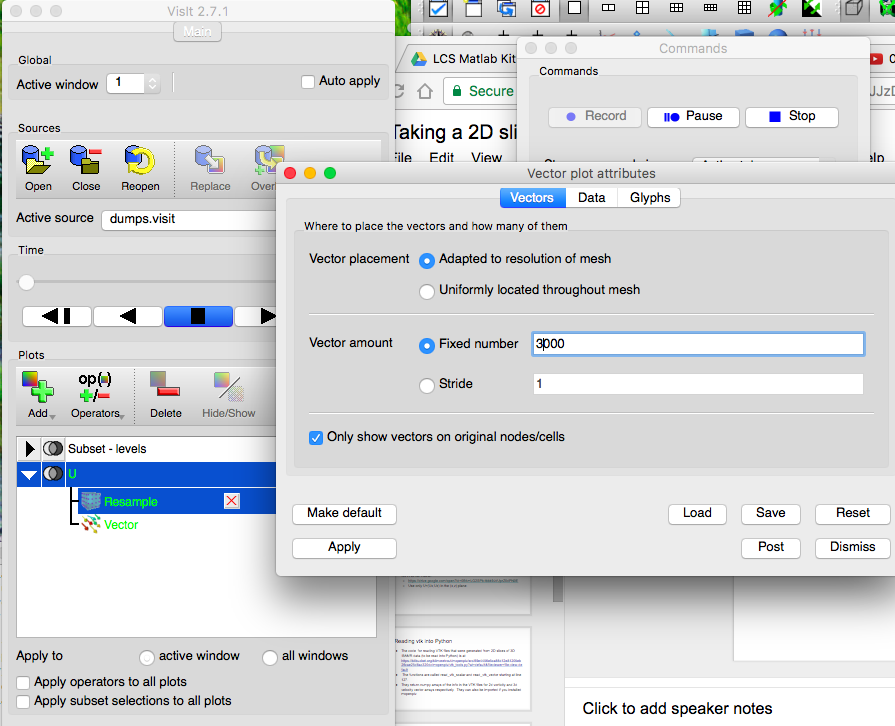
\includegraphics[width=0.9\textwidth]{ch33-d18-vector-attr.png}\\
\scriptsize ``Calculate the number of vectors you resampled. In this case it's 30x1x100=3000. Use that for the number of vectors.''
\column{0.4\textwidth}\centering
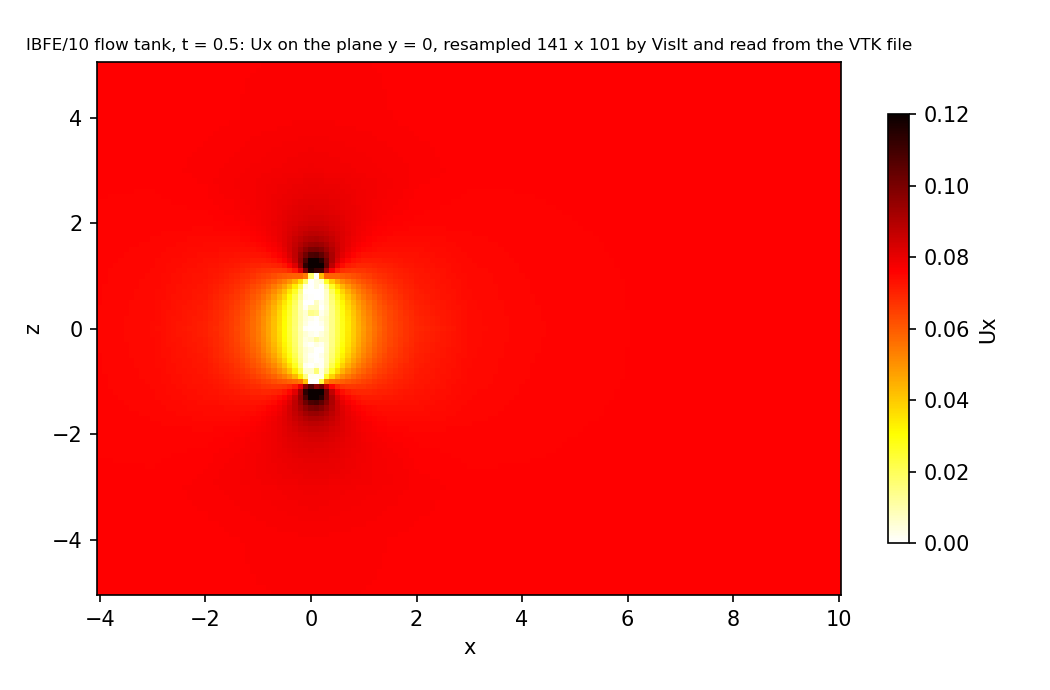
\includegraphics[width=0.9\textwidth]{ch33-ft-plane.png}\\
\scriptsize now: IBFE/10's flow tank, $U_x$ on $y = 0$ at $t = 0.5$, $141 \times 101$ samples, exported by \code{resample\_export.py} and read with \code{read\_vtk\_legacy.py}
\end{columns}
\footnotesize
\begin{itemize}
  \item ``You can't actually pick a 2D slice, but you can export only one value of x, y or z'': one sample in the normal direction (with the thin slab of slide \ref{fr:empty}) is the plane; the exported file is a \code{RECTILINEAR\_GRID} of \code{DIMENSIONS 141 1 101} with the vector at each point and \code{TIME} in its field data.
\end{itemize}
\sourcecredit{Left two: ``Taking a 2D slice from 3D IBAMR'' (2017), VisIt 2.7.1.}
\end{frame}

\begin{frame}{The same plane from the dumps, and when to use which}
\label{fr:plane2}
\footnotesize
\begin{itemize}
  \item The same plane straight from the dumps: \code{samrai\_dumps.py} in 3D fills the finest grid of the whole box (trilinear for nodal data), from which one slice is taken; for a $256^3$ run that is 16 M nodes per variable, so VisIt's resample of the plane alone is the lighter tool there.
\end{itemize}
\end{frame}

% 17
\begin{frame}[fragile]{Reading VTK in Python: three ways}
\label{fr:vtkpy}
\footnotesize
\begin{columns}[T]
\column{0.54\textwidth}
\begin{lstlisting}[style=tiny]
# vtk DataFile Version 4.2           <- what VisIt wrote (legacy ASCII)
vtk output
ASCII
DATASET RECTILINEAR_GRID
FIELD FieldData 3
MeshName 1 1 string
amr_mesh
CYCLE 1 1 int
19096
TIME 1 1 double
0.9548
DIMENSIONS 201 97 1
X_COORDINATES 201 double
0 0.03125 0.0625 ...
Y_COORDINATES 97 double
...
POINT_DATA 19497
SCALARS Omega double
LOOKUP_TABLE default
...                                  # one value per point, x fastest
\end{lstlisting}
\begin{lstlisting}[style=pytiny]
import read_vtk_legacy as rv                 # numpy only (examples/analysis)
v = rv.read_vtk("Omega_0056.vtk"); x, y, z = rv.grid_axes(v)
omega = v["data"]["Omega"]                   # (97, 201); vectors keep a last axis of 3
t = v["field"]["TIME"][0]
\end{lstlisting}
\column{0.44\textwidth}
\scriptsize
\begin{itemize}
  \item \al{No library:} \code{read\_vtk\_legacy.py} parses the legacy ASCII file into axes, point data (reshaped \code{[y, x]}), points and cells for the unstructured kinds (an exported Exodus mesh, Silo points), and the \code{FIELD} block (\code{TIME}, \code{CYCLE}).
\end{itemize}
\end{columns}
\end{frame}

\begin{frame}{Reading VTK in Python (2): the vtk module, pyvista, meshio}
\label{fr:vtkpy2}
\footnotesize
\begin{itemize}
  \item \al{The \code{vtk} module} (Strickland 2017, \code{read\_vtk\_data.py}): \code{vtkRectilinearGridReader} / \code{vtkStructuredPointsReader} / \code{vtkUnstructuredGridReader}, \code{numpy\_support.vtk\_to\_numpy}, the \code{dataset\_adapter} for \code{FieldData['TIME']}; reads binary legacy and, with the XML readers, \code{.vtr}. ``Because the vtk library is used to load the vtk file data, these functions should not be sensitive to line numbers or slight variation in format'' (his README). Indexed \code{[z, y, x]}.
  \item \al{\code{pyvista}} (\code{pyvista.read("file.vtr")}) when it is installed; \code{meshio} for files VisIt did not write (slide \ref{fr:empty}).
  \item The 2017 decks pointed at \code{mopenpiv/vtk\_tools.py} (``read\_vtk\_scalar and read\_vtk\_vector starting at line 127'') on Bitbucket, which is gone.
\end{itemize}
\end{frame}

% 18
\begin{frame}[fragile]{Reading VTK in MATLAB}
\label{fr:vtkm}
\footnotesize
\begin{columns}[T]
\column{0.5\textwidth}
\begin{lstlisting}[style=mtiny]
% examples/analysis/read_vtk_legacy.m (checked in Octave 8.4)
v = read_vtk_legacy('Omega_0056.vtk');
% v.type 'RECTILINEAR_GRID', v.dims [201 97 1], v.x, v.y, v.z
% v.data.Omega (97 x 201), v.field.TIME
pcolor(v.x, v.y, v.data.Omega); shading flat; axis equal
w = read_vtk_legacy('U_0056.vtk');           % w.data.U (97 x 201 x 3)
quiver(w.x, w.y, w.data.U(:,:,1), w.data.U(:,:,2))
\end{lstlisting}
\begin{lstlisting}[style=mtiny]
% N. Battista, 2017: read_Structured_Vector_Field_Data_From_vtk.m
strName = 'visit_ex_db';                 % the file, without .vtk
[U,V,W,X,Y,Z,Nx,Ny,Nz] = give_Me_The_Data_Please(strName);
% skips 5 header lines, sscanf('%*s %f %f %f %*s') for DIMENSIONS,
% fscanf the X, Y, Z coordinates, then 3*Nx*Ny*Nz numbers,
% reshape(U, Ny, Nx, Nz)
\end{lstlisting}
\column{0.48\textwidth}
\scriptsize
\begin{itemize}
  \item \code{read\_vtk\_legacy.m} reads the same headers as the Python version (\code{RECTILINEAR\_GRID}, \code{STRUCTURED\_POINTS}, \code{UNSTRUCTURED\_GRID}, \code{POLYDATA}; scalars and vectors; the \code{FIELD} block) and returns arrays indexed \code{(y, x)}; ASCII only (convert a binary export with VisIt's \gui{Legacy Ascii} option, or read it in Python).
  \item Nick Battista's 2017 reader is written for one layout, the \code{RECTILINEAR\_GRID} that VisIt 2.x exported from a 3D resample, with the line numbers of that file built in: it fails on a file with a \code{FIELD} block in front (VisIt 3 writes one) and on scalar exports (the \code{LOOKUP\_TABLE} line). Its \code{Convert\_vtk2LCS.m} loops over \code{visit\_ex\_db\_<k>.vtk}, reads each with the same function and writes \code{x z u w} text lines for Dabiri's LCS code (``Loop assumes we are looking at velocity data in the x,z-plane''). A note in it: the $Z$ loop reads \code{Nz} values with a format built for \code{Ny} (a copy slip; harmless, because \code{fscanf} recycles the format).
  \item The 2013 lecture's \code{pcolor\_frames.m} drew \code{Vinterp} this way; slide \ref{fr:frames} does it in Python.
\end{itemize}
\end{columns}
\end{frame}

% 19
\begin{frame}[fragile]{The ExodusII file in Python and MATLAB}
\label{fr:exodus}
\footnotesize
\begin{columns}[T]
\column{0.5\textwidth}
\begin{lstlisting}[style=tiny]
$ ncdump -h viz_IB2d/output.ex2            # netcdf-bin; IBFE/01 HALF
dimensions: time_step = UNLIMITED ; // (41 currently)
            num_dim = 2 ; num_nodes = 101 ; num_elem = 130 ;
            num_el_blk = 1 ; num_nod_per_el1 = 3 ; num_nod_var = 8 ;
variables:  double time_whole(time_step) ;
            double coordx(num_nodes) ; double coordy(num_nodes) ;
            int connect1(num_el_in_blk1, num_nod_per_el1) ;  // elem_type = "TRI3"
            char name_nod_var(num_nod_var, len_name) ;
            double vals_nod_var1(time_step, num_nodes) ; ... vals_nod_var8
\end{lstlisting}
\begin{lstlisting}[style=pytiny]
import read_exodus as rx                     # netCDF4
m = rx.Exodus("viz_IB2d/output.ex2")
m.nodal_names        # ['dX_0','dX_1','X_0','X_1','F_0','F_1','U_0','U_1']
m.var("dX_1", 10)[0] # 0.500402: node 0 at t = 1 (chapter 28's PickByNode, HALF run)
m.positions(10)      # coords + dX: equals (X_0, X_1) to 1e-16
m.connect["1"]       # (130, 3) 0-based triangles
\end{lstlisting}
\column{0.48\textwidth}
\scriptsize
\begin{itemize}
  \item ExodusII is netCDF with a fixed vocabulary: \code{coordx}, \code{coordy}, one \code{connect<b>} per element block, the names in \code{name\_nod\_var} (fixed-width characters), the fields as \code{vals\_nod\_var<k>(time\_step, num\_nodes)}. \code{ncdump -h} shows it all; \code{file} calls it HDF5 because netCDF-4 is HDF5 underneath (so \code{h5py} opens it too, without the names' meaning).
\end{itemize}
\end{columns}
\end{frame}

\begin{frame}[fragile]{The ExodusII file (2): MATLAB, and the plate's tips}
\label{fr:exodus2}
\footnotesize
\begin{columns}[T]
\column{0.5\textwidth}
\begin{lstlisting}[style=mtiny]
ex = read_exodus('viz_IB2d/output.ex2');     % ncread; Octave: pkg load netcdf
a = ex.var('dX_1', 11);  a(1)                % 0.500402 (1-based state and node)
p = ex.positions(11);  tri = ex.connect1;    % triplot(tri, p(:,1), p(:,2))
\end{lstlisting}
\begin{center}
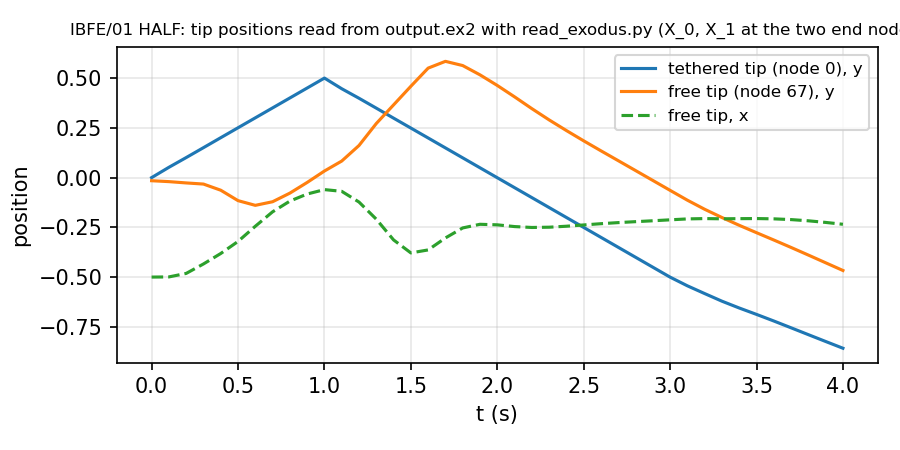
\includegraphics[width=\textwidth]{ch33-exodus-tips.png}
\end{center}
\column{0.48\textwidth}
\scriptsize
\begin{itemize}
  \item \code{read\_exodus.py} (Python, \code{netCDF4}) and \code{read\_exodus.m} (MATLAB's \code{ncread}; Octave's \code{netcdf} package, \code{apt install octave-netcdf}) give the times, the reference coordinates, the connectivity, any nodal field at one state or all, and the current configuration. Checked against chapter 28's \code{PickByNode} on the HALF run (both languages); the Pick printed in chapter 28 is the FULL run (0.500316).
  \item The tips of the HALF plate from the file (right): the tethered tip follows the prescribed path, the free tip swings behind it; the README's numbers of chapter 17 came from this.
\end{itemize}
\end{columns}
\end{frame}

% 20
\begin{frame}[fragile]{The Silo points: through VisIt, or from the \code{X} files}
\label{fr:silo}
\footnotesize
\begin{columns}[T]
\column{0.5\textwidth}
\begin{lstlisting}[style=pytiny]
# VisIt CLI: the point mesh of frame 56 as a VTK file
OpenDatabase("viz_IB2d/lag_data.visit"); DeleteAllPlots()
AddPlot("Mesh", "human_vertices"); DrawPlots(); SetTimeSliderState(56); DrawPlots()
e = ExportDBAttributes(); e.db_type = "VTK"; e.db_type_fullname = "VTK_1.0"
ExportDatabase(e, GetExportOptions("VTK"))         # -> <cwd>/.vtk, rename it
\end{lstlisting}
\begin{lstlisting}[style=pytiny]
v = rv.read_vtk("points_0056.vtk")                # UNSTRUCTURED_GRID / POLYDATA
pts = v["points"][:, :2]                          # (1045, 2)
X = hd.read_vec("hier_data_IB2d/X.19096")         # chapter 11's reader, same step
abs(pts - X[:, :2]).max()                         # 1.0e-5 cm: the Silo file's single precision
\end{lstlisting}
\column{0.48\textwidth}
\scriptsize
\begin{itemize}
  \item The \code{lag\_data} files are Silo with the PDB driver (\code{DBCreate(..., DB\_PDB)} in \code{LSiloDataWriter.cpp}): not HDF5, so \code{h5py} refuses them, and there is no Silo reader in a plain Python. VisIt reads them, and \gui{Export Database} with the Mesh plot active writes the points (and the spring edges from \code{<name>\_mesh}) as VTK, one state at a time (slide \ref{fr:empty}).
  \item Simpler: the \code{X.NNNNN} text files of chapter 11 hold the same positions in double precision at the \code{data\_dump\_interval}; with equal intervals (the inputs of this series) the step numbers match frame for frame, as the check at left shows (the difference is the Silo file's single precision). Forces are only there.
  \item Silo's own Python module comes with the Silo library when it is built with Python support (VisIt 3.5.0's Linux tarball does not include it); chapter 32 uses it if a reader without VisIt is ever needed.
\end{itemize}
\end{columns}
\end{frame}

% 21
\begin{frame}[fragile]{The HDF5 state dumps of the upstream examples}
\label{fr:hierh5}
\footnotesize
\begin{columns}[T]
\column{0.56\textwidth}
\begin{lstlisting}[style=tiny]
PatchHierarchy/                                    # hier_data.00033.samrai.00000
  d_number_levels [3]
  level_0000/  d_boxes, d_ratio_to_coarser_level, d_number_patches ...
    level_0000-patch_0000/
      INSStaggeredHierarchyIntegrator::P##INSStaggeredHierarchyIntegrator::CURRENT/
        d_box, d_ghost_box, d_ghosts [0 0], d_depth [1]
        d_data/d_array (512,) >f8               # cell data, 8 x 64: no ghost cells in these dumps
      INSStaggeredHierarchyIntegrator::U##INSStaggeredHierarchyIntegrator::CURRENT/
        d_data0/d_array (520,)  d_data1/d_array   # side data: x faces, y faces
      PolymericStressForcing::C_cc##AdvDiffSemiImplicitHierarchyIntegrator::CURRENT/
        d_data/d_array, d_depth [3]              # a tensor, depth 3
\end{lstlisting}
\begin{lstlisting}[style=pytiny]
import hier_data_h5 as hd5
f = hd5.HierData("hier_data_IB2d/hier_data.00033.samrai.00000")
f.variables                      # the three names above
for p in f.patches(f.variables[0]):
    p["level"], p["lo"], p["hi"], p["data"]      # P: [y, x] without ghosts
# U: p["data"] = [u on the x faces (ny, nx+1), v on the y faces (ny+1, nx)]
\end{lstlisting}
\column{0.42\textwidth}
\scriptsize
\begin{itemize}
  \item IBAMR's own \code{examples/IB/explicit/ex1} (chapter 11's writer descends from it), the IBFE examples and the complex-fluids ones write, every \code{data\_dump\_interval}, the solver's state through SAMRAI's HDF5 database: one file per rank, the hierarchy, and per patch every registered variable with its context (\code{\#\#CURRENT}), its box, its ghost width and its depth.
\end{itemize}
\end{columns}
\end{frame}

\begin{frame}{The HDF5 state dumps, continued}
\label{fr:hierh52}
\footnotesize
\begin{itemize}
  \item These are the real arrays: double precision, \code{P} cell-centred, \code{U} side-centred (the $x$ component on the $x$ faces: \code{(ny, nx+1)}), with \code{d\_ghosts} ghost cells around them when the writer adds any (these dumps have none: \code{d\_ghosts [0 0]}, and $512 = 8 \times 64$). \code{hier\_data\_h5.py} strips the ghosts, if present, and returns each patch; the output above is from the complex-fluids \code{ex2} run of chapter 25 (16 patches on 3 levels; the polymeric stress tensor as a depth-3 field).
  \item Reading them is the way to check a solver quantity VisIt's nodal copies blur (\code{Div U} at the cell centres, the staggered velocity); the series' examples do not write them (slide \ref{fr:check}).
\end{itemize}
\end{frame}

% 22
\begin{frame}[fragile]{Curves, and the lists after a restart}
\label{fr:curves}
\footnotesize
\begin{columns}[T]
\column{0.5\textwidth}
\begin{lstlisting}[style=mtiny]
C = importdata('plate_dX_queries.curve');  % one block per curve (chapter 28)
t = C.data(:,1); y = C.data(:,2);
\end{lstlisting}
\begin{lstlisting}[style=shell]
# chapter 3: after a restart, dumps.visit lists only the new frames
$ wc -l dumps.visit.after_restart dumps.visit      # 35 vs 77 in the test run
$ ls -d visit_dump.* | sort -t. -k2 -n | sed 's#$#/summary.samrai#' > dumps.visit
$ for d in $(ls -d lag_data.cycle_* | sort -t_ -k3 -n); do echo "$d/$d.summary.silo"; done > lag_data.visit
\end{lstlisting}
\begin{lstlisting}[style=pytiny]
frames = sd.frames("viz_IB2d")        # reads dumps.visit: rebuild it first
\end{lstlisting}
\column{0.48\textwidth}
\scriptsize
\begin{itemize}
  \item \code{.curve} files (queries over time, picks with a time curve, lineouts) are text with a \code{\#} header per curve; chapter 28's slide has the MATLAB and Python readers; Lindsay Waldrop's 2017 note on batch processing adds that they ``are pretty easy to import into R''.
  \item A restarted run truncates \code{dumps.visit} and \code{lag\_data.visit} to the frames after the restart (chapter 3's test: 35 lines for 77 folders on disk); the readers of this chapter trust the lists (\code{sd.frames} walks \code{dumps.visit}), so rebuild them with chapter 3's two lines before an analysis spanning the restart. The Exodus file of an IBFE run is one file and \code{append(from\_restart)} keeps it whole (chapter 17).
  \item The frame times are in the files (\code{BASIC\_INFO/time}, \code{time\_whole}), not in the lists; \code{sd.frames} returns them.
\end{itemize}
\end{columns}
\end{frame}

% 23
\begin{frame}{The 2020 lecture's Eulerian analysis: \code{flappy\_ends.m} and \code{vol\_flow\_rate.m}}
\label{fr:lecture}
\begin{columns}[T]
\column{0.42\textwidth}\centering
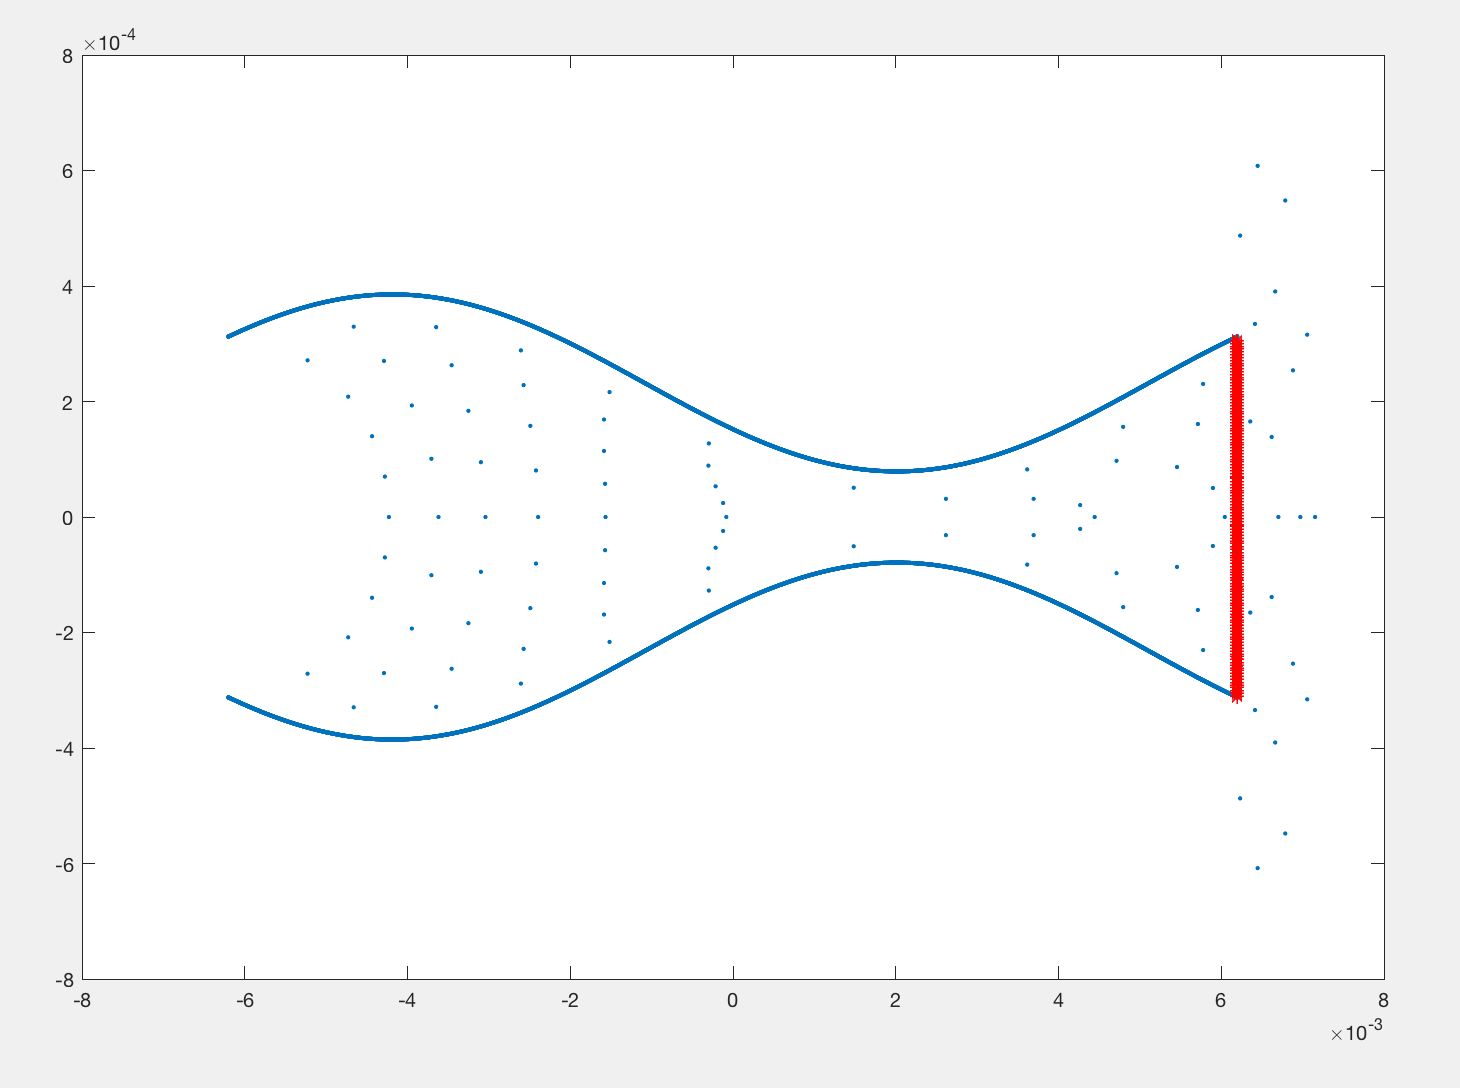
\includegraphics[width=0.9\textwidth]{ch33-l20-tube-line.png}\\
\scriptsize ``The figure that is generated shows the tube (blue) and the line over which the volumetric flux is calculated (red).''
\column{0.56\textwidth}
\footnotesize
\begin{itemize}
  \item ``This function imports SAMRAI data into Matlab, interpolates to a uniform grid, reads in the lagrangian positions, and calculates the volumetric flow rate and maximum velocity at the end of the tube'' (\code{flappy\_end\_analysis}, 2020). Its inputs were typed at the top of the script: \code{GridSizex = 4096}, \code{GridSizey = 512} (``size of the finest grid''), \code{starting\_time = 10000}, \code{time\_step = 5000} (``this should match the interval in the input2d file''), \code{final\_time = 55000}, \code{timestep = 7.5e-6} (``dt used in IBAMR''), \code{Lminx = -0.01} \ldots, \code{pperitop = 5080} (``the number of points along the top of the tube'').
\end{itemize}
\end{columns}
\sourcecredit{``5 -- Reading forces and converting IBAMR output to Matlab'' (2020), slides 15--20 and the figure of slide 17.}
\end{frame}

\begin{frame}{The 2020 lecture's flow-rate function, and what replaces its hand-typed inputs}
\label{fr:lecture2}
\footnotesize
\begin{itemize}
  \item \code{vol\_flow\_rate.m} ``returns the volumetric flow rate across the end of the tube and the maximum velocity along the end of the tube at the given instance in time'', with the row and column indices it used; the run was ``a long heart tube with contraction prescribed as a traveling sine wave''; ``the volumetric flow rate in m$^3$/s'' is, in 2D, a rate per unit depth.
  \item The pattern, grid size and interval copied by hand from the input file, is what \code{samrai\_dumps.py} reads from the files instead (slide \ref{fr:flow}).
\end{itemize}
\end{frame}

% 24
\begin{frame}[fragile]{The flow rate across a line, now: \code{flow\_rate.py}}
\label{fr:flow}
\footnotesize
\begin{columns}[T]
\column{0.5\textwidth}
\begin{lstlisting}[style=tiny]
$ python3 flow_rate.py viz_IB2d x=-1.5,0.0,1.5 y=-0.5:0.5 out=flux.csv plot=flux.png
time,x=-1.5,x=0,x=1.5
0,0,0,0
0.005,0.3433,0.1929,0.3429
...
0.25,0.7125,0.7374,0.7126
# mean over the frames: x=-1.5: 0.3726, x=0: 0.3730, x=1.5: 0.3726
\end{lstlisting}
\begin{center}
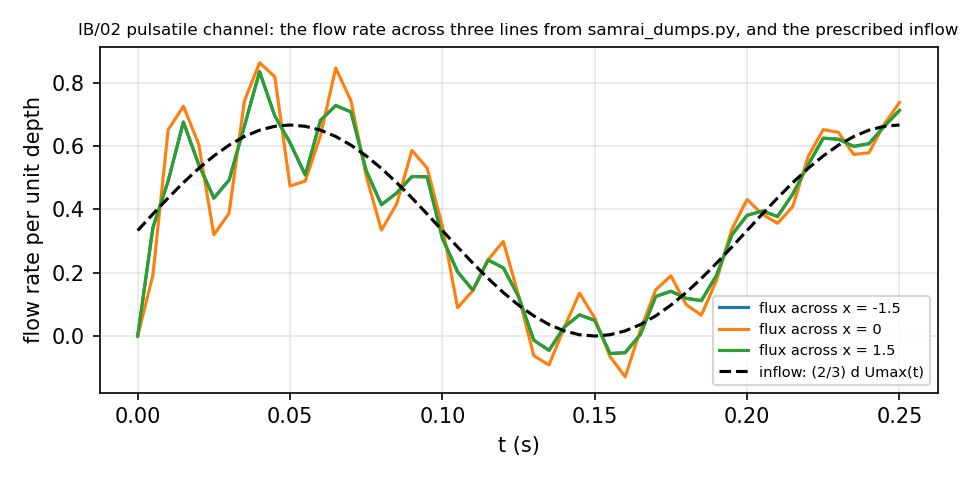
\includegraphics[width=0.95\textwidth]{ch33-flux-channel.png}
\end{center}
\column{0.48\textwidth}
\scriptsize
\begin{itemize}
  \item \code{flow\_rate.py} walks \code{dumps.visit}, puts \code{U} on the finest grid at each frame and integrates $u$ across each line (trapezoid rule after a linear interpolation in $x$; \code{line\_flux} in \code{samrai\_dumps.py}); horizontal lines take $v$.
\end{itemize}
\end{columns}
\end{frame}

\begin{frame}{The flow rate across a line: what the numbers say}
\label{fr:flow2}
\footnotesize
\begin{itemize}
  \item IB/02, the pulsatile channel (chapter 7's $0.25$ s run, 51 frames, $512^2$ finest grid): the flow rates across $x = -1.5$ and $x = 1.5$ agree with one another to $0.0017$ over the whole run and to $0.0004$ after $0.15$ s ($0.05$ \% of the peak $0.83$): incompressibility, checked. The line at $x = 0$ differs from them by up to $0.16$ ($0.077$ after $0.15$ s, 9 \% of the peak; the listing shows it): it crosses the refined region around the channel, and the cause was not run down. Report the lines you trust and say why.
  \item Against the prescribed inflow, $Q_\mathrm{in} = \frac{2}{3} d\,U_\mathrm{max}(t)$ with $U_\mathrm{max} = \frac12 + \frac12 \sin(2\pi\,5\,t)$ (the parabola of chapter 7's \code{gcoef} integrated over $|y| < d/2$): a start-up transient (the run begins at rest with the inflow already at $Q = 1/3$), then the outer lines within $0.07$ (8 \% of the peak) after $0.15$ s; the point walls are not sealed, and the box around the channel is open. The means over the 51 frames, $0.3726$ ($x = \pm 1.5$) against $0.3781$; over frames 1--50 ($t > 0$), $0.380$ against $0.379$.
\end{itemize}
\end{frame}

% 25
\begin{frame}{The flow rate of the valveless pump (IB/11)}
\label{fr:pump}
\begin{columns}[T]
\column{0.5\textwidth}\centering
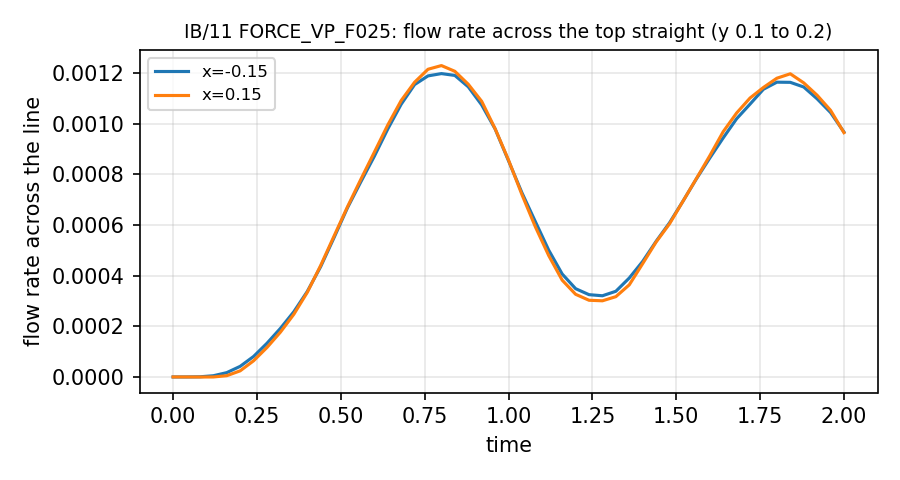
\includegraphics[width=0.95\textwidth]{ch33-flux-pump.png}\\
\scriptsize IB/11 \code{FORCE\_VP\_F025} (chapter 9b's shipped suction run): the flow rate across the loop's top straight (the rigid side opposite the elastic section) at $x = -0.15$ and $x = 0.15$ m, $y \in [0.1, 0.2]$, over two periods (51 frames).
\column{0.48\textwidth}
\footnotesize
\begin{itemize}
  \item The two lines give the same curve (means $6.64$ and $6.65 \times 10^{-4}$ m$^2$/s): the flux along the tube is one number at each instant.
  \item The mean, $6.6 \times 10^{-4}$ m$^2$/s per unit depth through a $0.1$ m tube, is a mean speed of $6.6$ mm/s in the $+x$ direction along the top, so the loop turns clockwise and the flow along the elastic section is in $-x$ (chapter 29 finds the same flux on both bends and across the whole pericardium), pumped by a squeeze that never closes the tube: Liebau's valveless pumping, measured as a flux. Chapter 9b's README measured the markers' drift in the elastic section, $+1.1$ and $+1.0$ cm per period: against the net flow there. A drift of marker points is not a flux.
\end{itemize}
\end{columns}
\end{frame}

\begin{frame}{The pump's flow rate (2): where to put the line}
\label{fr:pump2}
\footnotesize
\begin{itemize}
  \item A line across the lower, elastic section at $x = -0.15$, between the walls' rest positions, gave almost nothing, probably because the tube moves, bulging past such a line in places and narrowing inside it in others, so the line crosses part of the tube and part of the gap between tube and pericardium. Across the whole pericardium ($y$ from $-0.245$ to $-0.055$) the flux is the loop's again, $6.6 \times 10^{-4}$ m$^2$/s in $-x$ (chapter 29); check the geometry before trusting a line (chapter 9b's figures show where the tube is).
  \item The same loop over \code{sd.frames} gives any other quantity: the maximum speed on the line, the mean pressure drop between two lines, the kinetic energy in a box.
\end{itemize}
\end{frame}

% 26
\begin{frame}{Frames and positions together: \code{pcolor\_frames.m} in Python}
\label{fr:frames}
\begin{center}
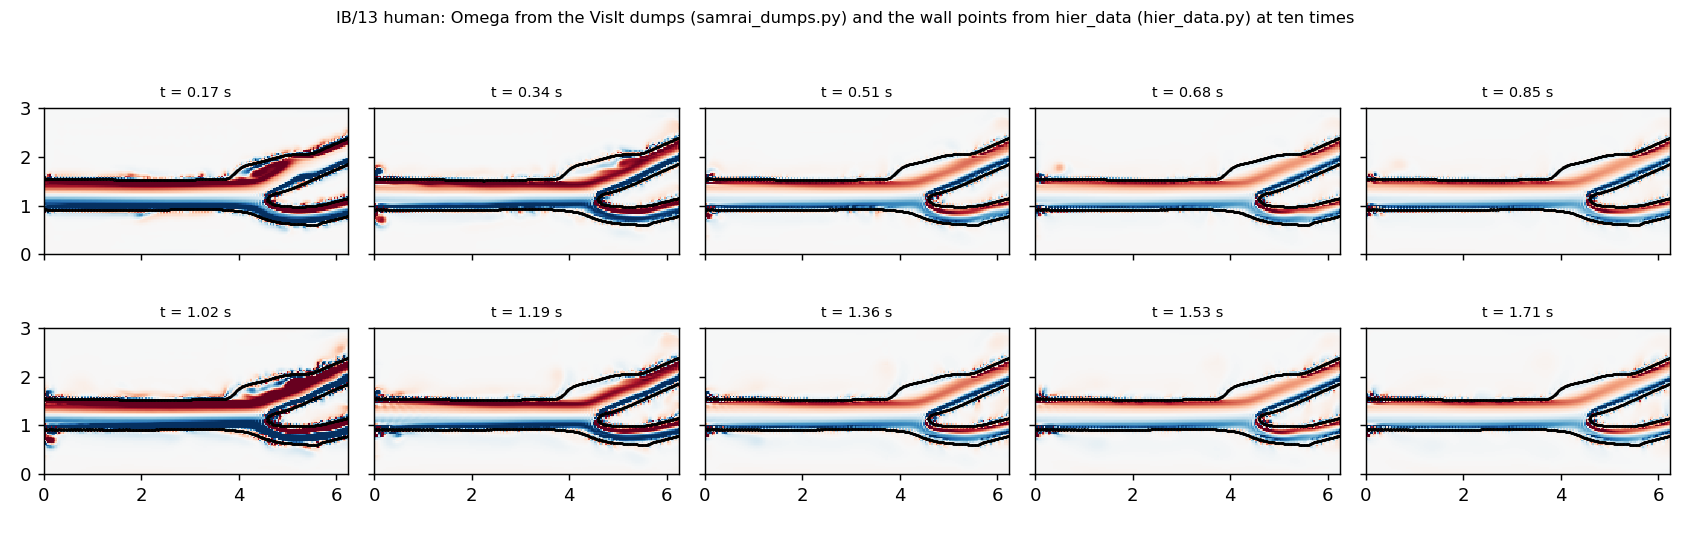
\includegraphics[width=0.84\textwidth]{ch33-py-frames.png}
\end{center}
\footnotesize
\begin{itemize}
  \item The 2013 lecture's \code{pcolor\_frames.m}, in the words of its header (spelling corrected): reads positions from \code{hier\_data} and vorticities from the \code{viz\_IB2d} SAMRAI data and makes a $5 \times 2$ plot of vorticity at 10 times; it is specific to jellyfish swimming, in that the $y$ position of the top of the bell is read and all $y$ values are shifted so that the top of the bell is always at $y = 0$. Its output and the position and velocity plots of \code{readpositions.m} are three of the four figure slides of that lecture (slide \ref{fr:lecturefigs}).
  \item The same in 30 lines (\code{tools/ch33\_frames.py}): \code{sd.frames}, \code{d.uniform("Omega")} and \code{pcolormesh} for the field, \code{hier\_data.read\_vec("X.<step>")} (chapter 11) for the points of the same step, a $2 \times 5$ grid of axes.
\end{itemize}
\end{frame}

% 27
\begin{frame}{The 2013 lecture's figures}
\label{fr:lecturefigs}
\begin{columns}[T]
\column{0.44\textwidth}\centering
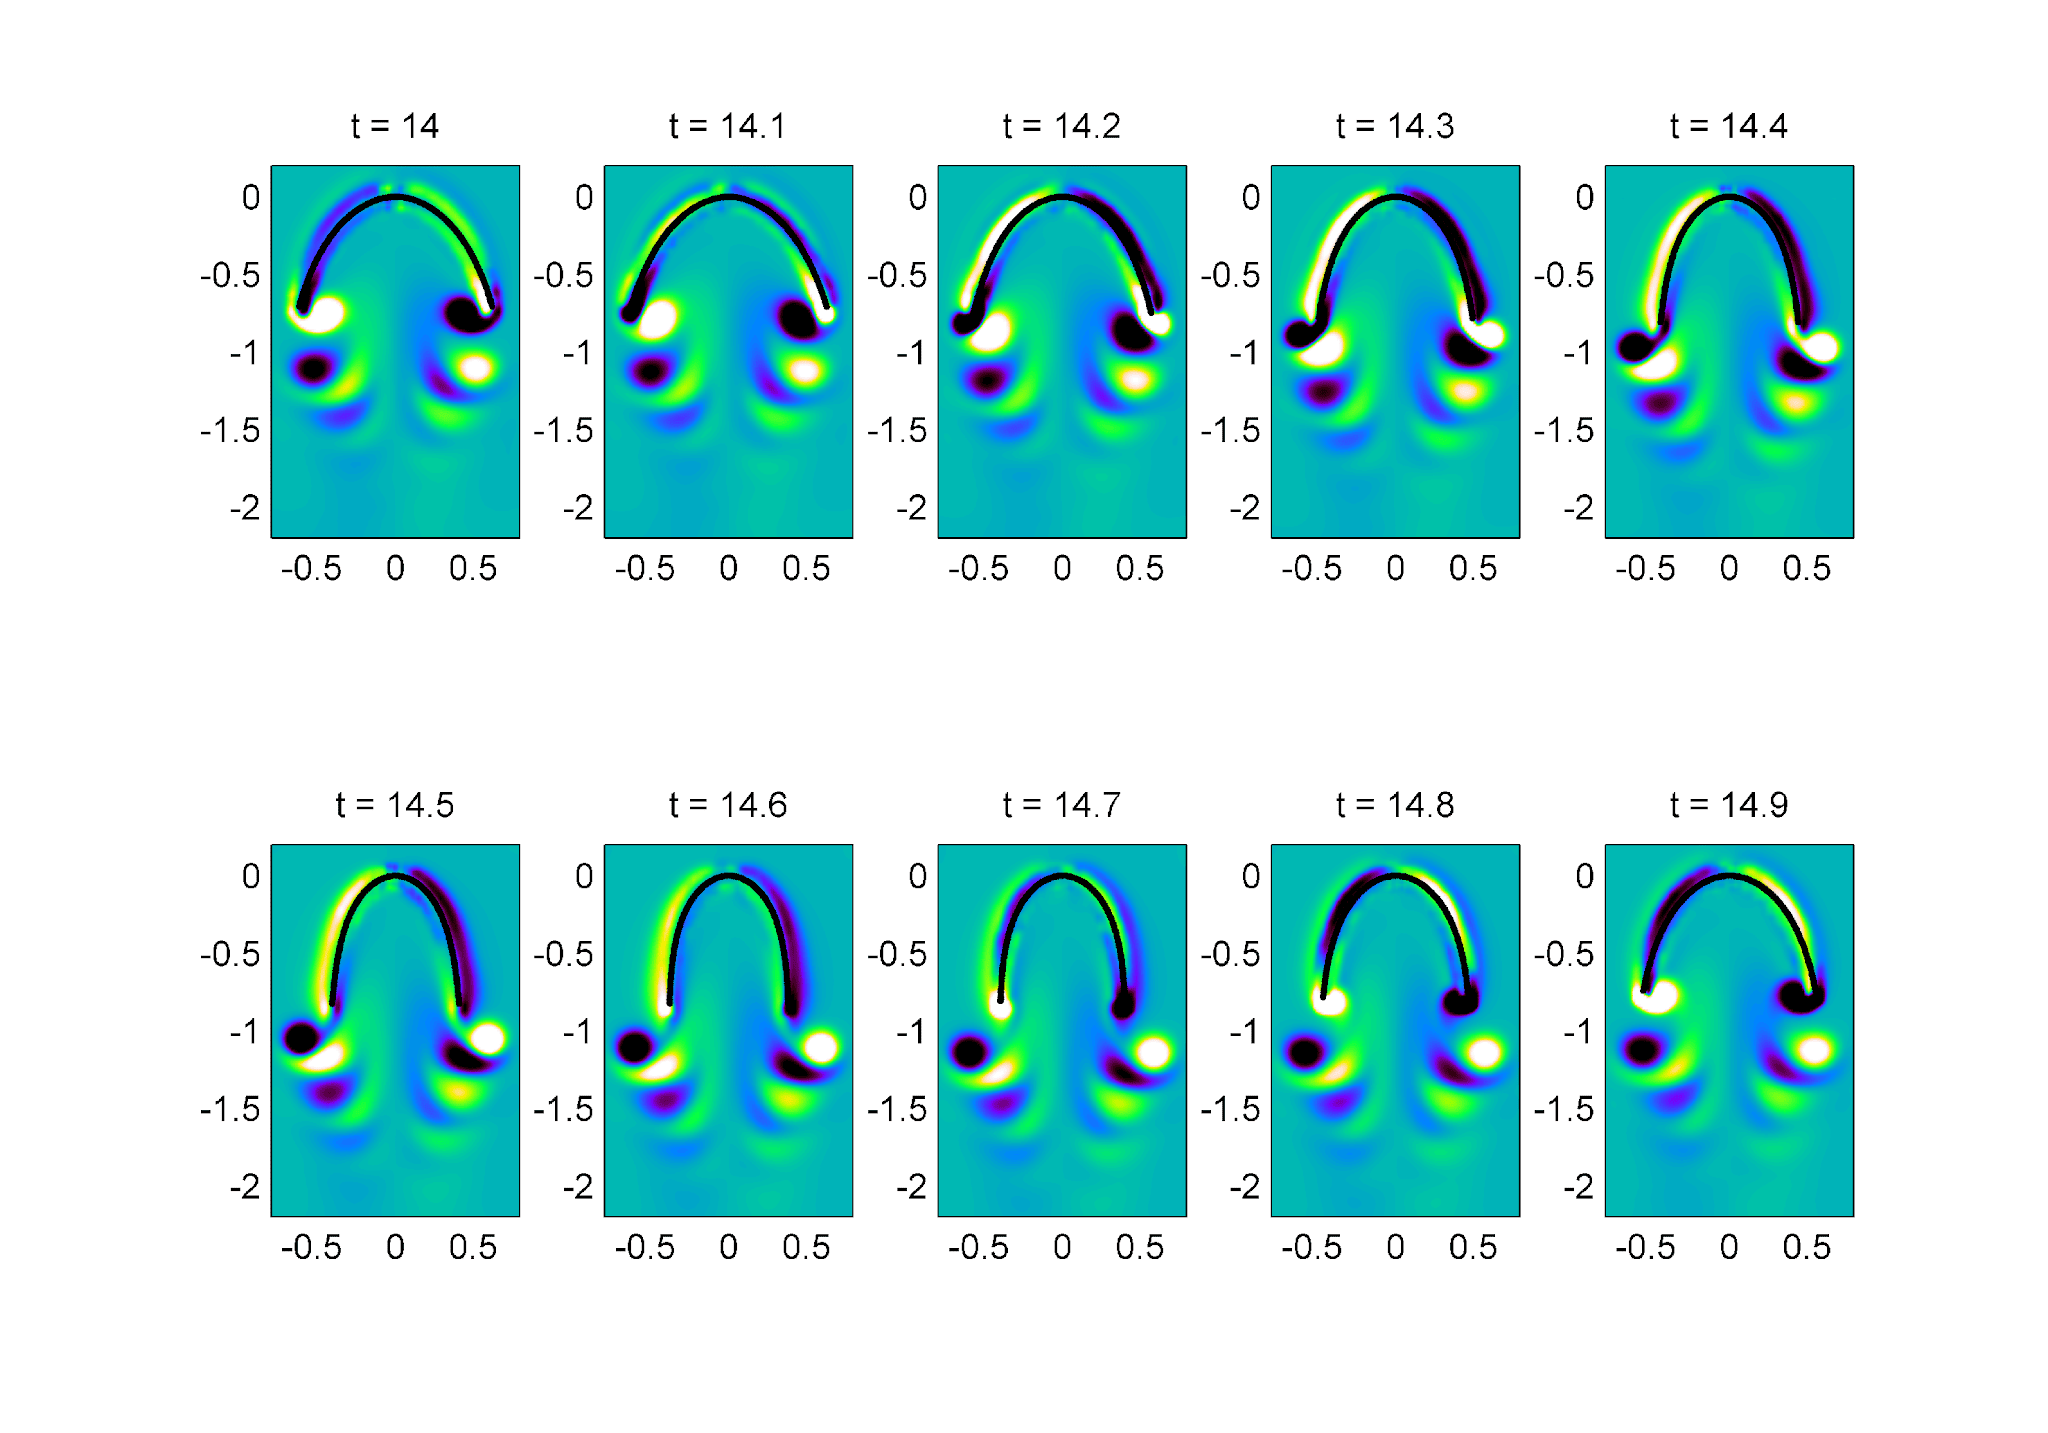
\includegraphics[width=\textwidth]{ch33-l20-pcolor-frames.png}\\
\scriptsize ``Plots generated by pcolor\_frames'': a jellyfish bell at $t = 14$ to $14.9$
\column{0.27\textwidth}\centering
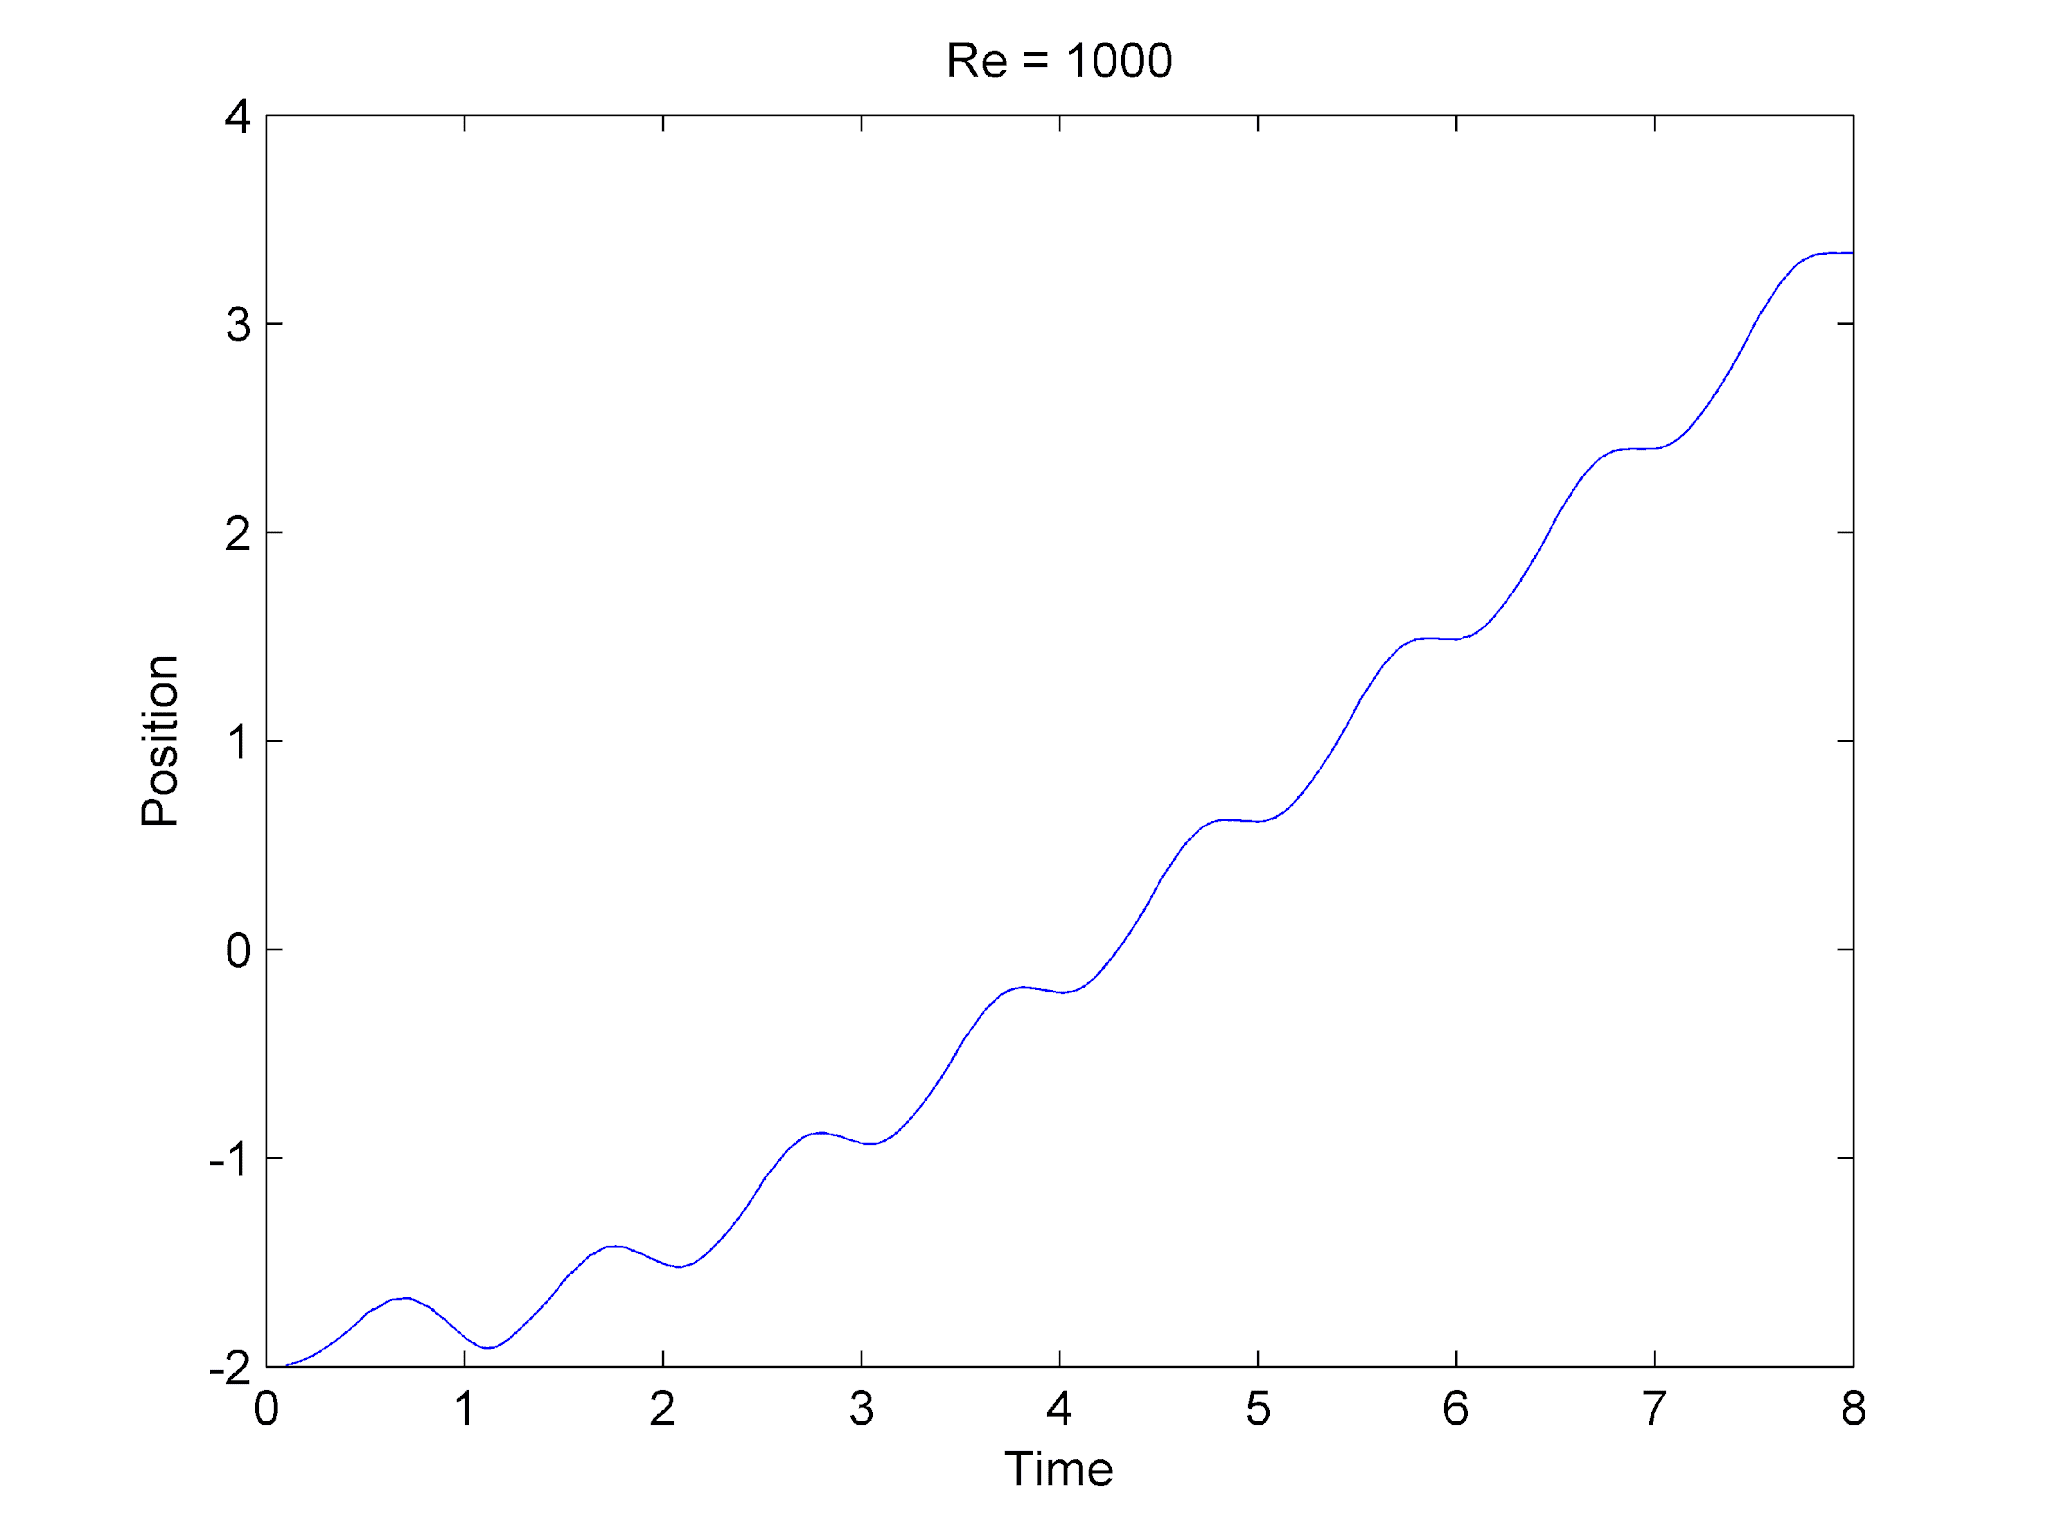
\includegraphics[width=\textwidth]{ch33-l20-position.png}\\
\scriptsize ``Plots generated from readpositions.m'': the bell's position, $\mathrm{Re} = 1000$
\column{0.27\textwidth}\centering
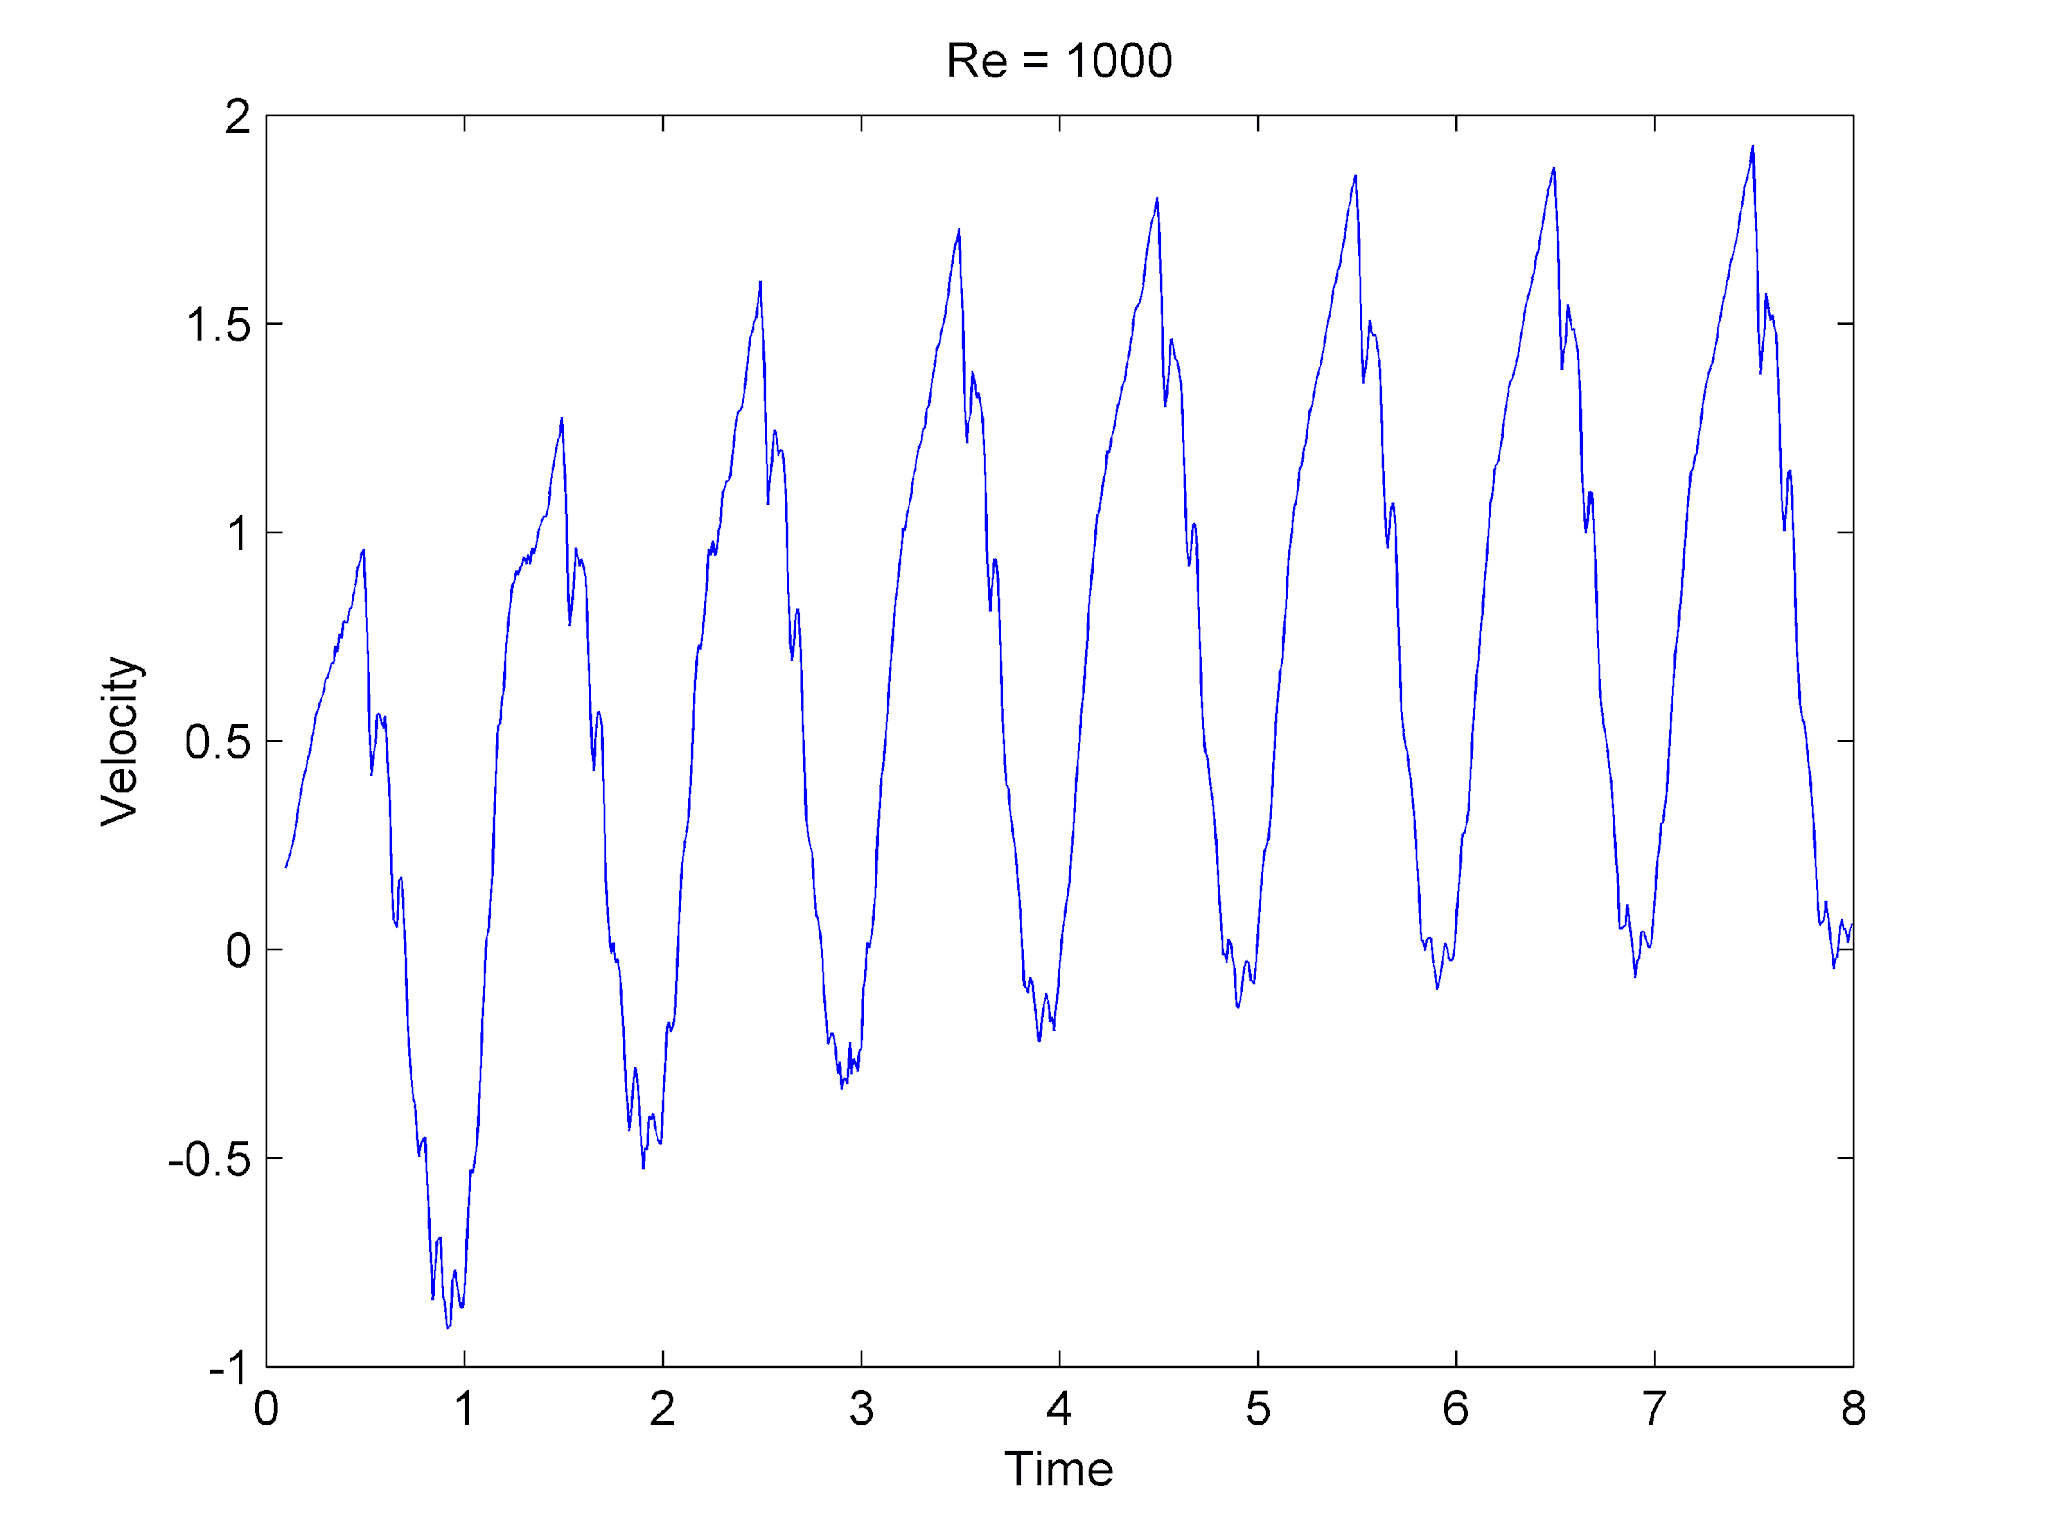
\includegraphics[width=\textwidth]{ch33-l20-velocity.png}\\
\scriptsize its velocity against time
\end{columns}
\footnotesize
\begin{itemize}
  \item The position and velocity of the bell's top against time, read from the \code{X} files and differentiated: chapter 11's \code{read\_series} does the reading, \code{numpy.gradient} the rest; chapter 10's IB/10 bell is the modern run.
  \item \code{Force\_vs\_time.m} of the same lecture (``the force on each boundary point is summed'', rescaled by $\rho S U^2$) is chapter 11's \code{leaf\_forces.py}.
\end{itemize}
\sourcecredit{``Converting IBAMR output to Matlab and analyzing it'' (MATH 769, 2013) and the 2020 re-issue: figure slides 10--12 / 23--24.}
\end{frame}

% 28
\begin{frame}[fragile]{PIV into VisIt: \code{piv\_to\_vtk.py}}
\label{fr:piv}
\footnotesize
\begin{columns}[T]
\column{0.5\textwidth}
\begin{lstlisting}[style=tiny]
$ python3 piv_to_vtk.py Vx.txt Vy.txt piv_field.vtk --dx 0.125 --dy 0.125 --flip
wrote piv_field.vtk: 51 x 25 vectors, spacing 0.125 x 0.125, |U| up to 109.8
\end{lstlisting}
\begin{lstlisting}[style=tiny]
# vtk DataFile Version 3.0
PIV vector field
ASCII
DATASET STRUCTURED_POINTS
DIMENSIONS 51 25 1
ORIGIN 0 0 0
SPACING 0.125 0.125 1
POINT_DATA 1275
VECTORS U double
0.0 0.0 0.0 ...
\end{lstlisting}
\begin{center}
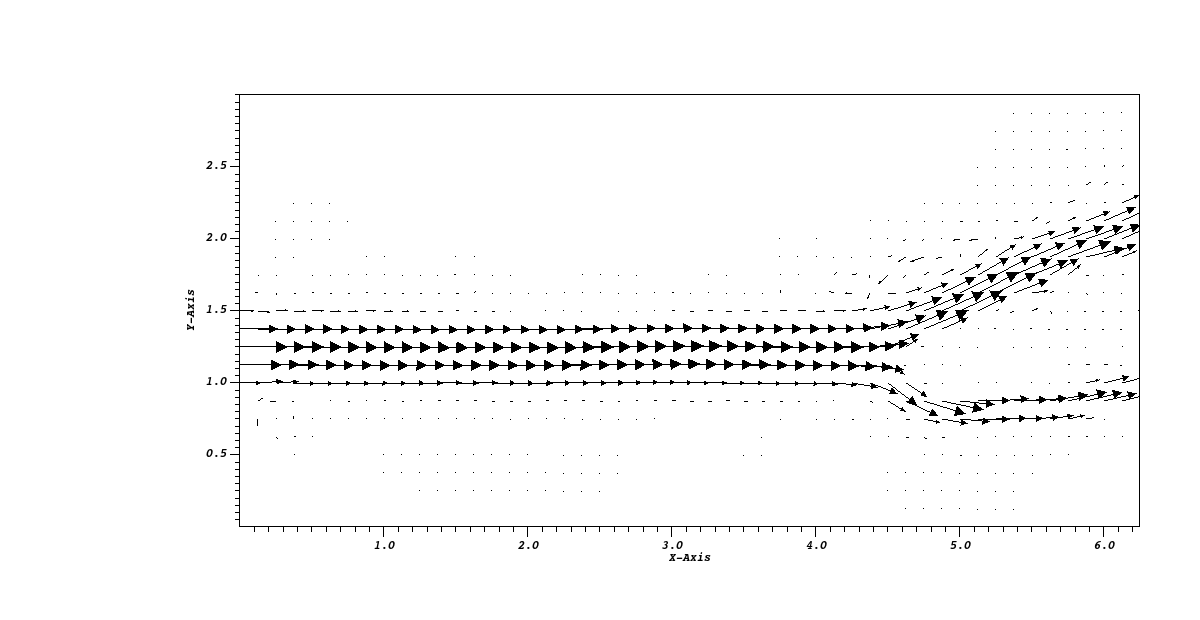
\includegraphics[width=0.7\textwidth]{ch33-piv-vtk.png}
\end{center}
\column{0.48\textwidth}
\scriptsize
\begin{itemize}
  \item The 2019 PIV document (old notes credited to ``Steve''): in DaVis, ``extract scalar field: vector component'' for $V_x$ and $V_y$ ``separately one at a time'', export each frame as ASCII text, then ``the python script toVTK.py (found in scripts/forPIV)'' turns the two files into a VTK file ``which can then be opened in VisIT''. That script is lost; \code{piv\_to\_vtk.py} is its replacement: two text arrays (rows $= y$, columns $= x$; DaVis, OpenPIV or NumPy), the spacing and origin, \code{--flip} when the first row is the top of the image.
  \item The output is a \code{STRUCTURED\_POINTS} vector field, the format IB2d writes too: VisIt's Vector and Pseudocolor plots, \code{magnitude(U)}, \code{U[0]}, and the LCS operator (FTLE is one of its outputs) take it as they take an IBAMR field; the picture is a test field (IB/13's velocity subsampled every fourth node) drawn by VisIt from the file.
  \item \code{write\_vtk\_vector(path, u, v, dx, dy)} in the same file writes any gridded field you compute in Python for VisIt.
\end{itemize}
\end{columns}
\end{frame}

% 29
\begin{frame}{PIV processing as the 2019 document showed it}
\label{fr:davis}
\begin{columns}[T]
\column{0.5\textwidth}\centering
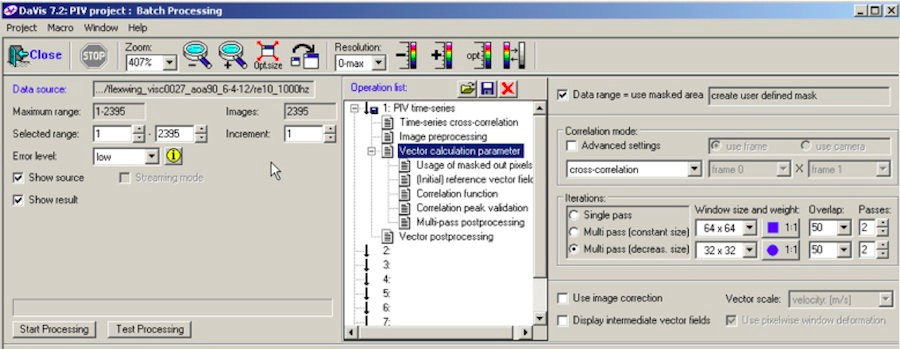
\includegraphics[width=0.9\textwidth]{ch33-davis-batch.png}\\
\scriptsize DaVis 7.2: \gui{F(batch)}, ``PIV -- time series'' with a multi-pass of decreasing window size, $64 \times 64$ to $32 \times 32$
\column{0.5\textwidth}\centering
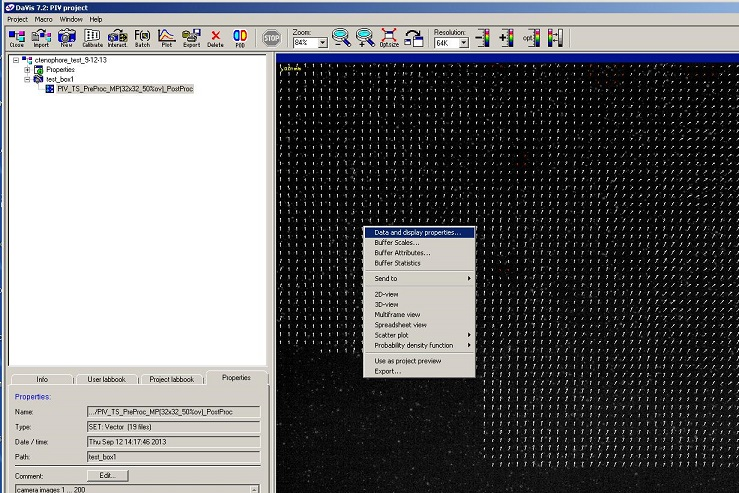
\includegraphics[width=0.9\textwidth]{ch33-davis-project.png}\\
\scriptsize the project window with a vector field below its image set; ``Data and display properties'' to scale the vectors
\end{columns}
\footnotesize
\begin{itemize}
  \item The document's recipe: highlight the image set, \gui{F(batch)}, choose ``PIV -- time series'' (``no pre-processing, no post-processing, and a multi-pass of decreasing size, 64x64 -- 32x32''), ``choose the range of images you want and the increment \ldots such that the particles move a few pixels with each image step'', start processing; then scale the display (``Data and display properties'', vector length, vector colour range).
\end{itemize}
\sourcecredit{``6. Analyze PIV Data'' (2019 lab document), DaVis 7.2 screenshots.}
\end{frame}

\begin{frame}{PIV processing (2): what the document left to do, and OpenPIV}
\label{fr:davis2}
\footnotesize
\begin{itemize}
  \item Its to-do list (``write a tutorial on how to use the MATLAB script on the PIV computer to export to .mat files'', ``find the files that convert ASCII text to .vtk from Steve'') is what the previous slide closes; the comparison of PIV fields with IBAMR fields (averages, circulation, LCS) is chapter 29.
  \item OpenPIV (the 2017 instructions by Julia Samson, E11; the \code{mopenpiv} fork is gone) is the open route to the vector fields; DaVis the commercial one (its batch window on the previous slide).
\end{itemize}
\end{frame}

% 30
\begin{frame}{Other programs' output into VisIt: COMSOL's VTU}
\label{fr:comsol}
\begin{columns}[T]
\column{0.5\textwidth}\centering
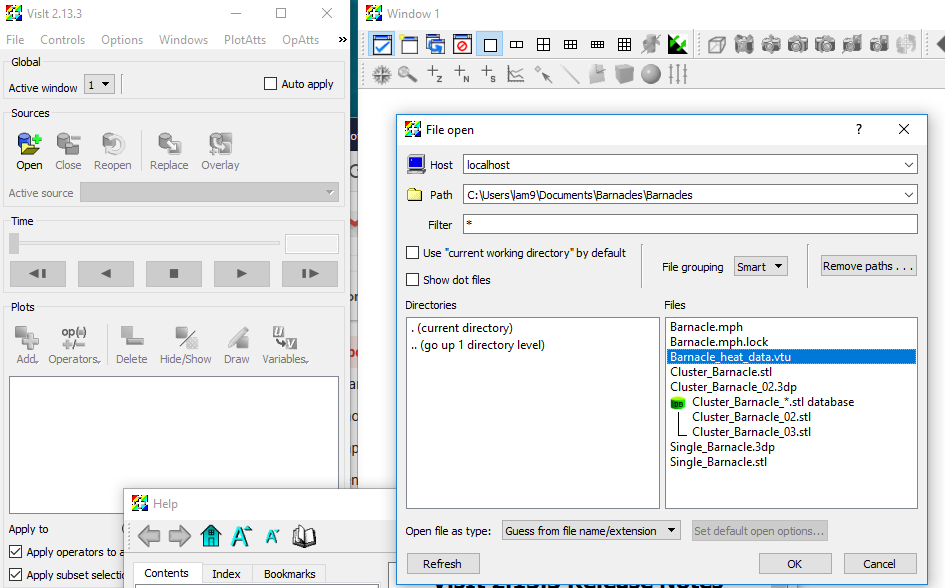
\includegraphics[width=0.6\textwidth]{ch33-comsol-visit-open.png}\\
\scriptsize VisIt 2.13.3 (Windows) opening \code{Barnacle\_heat\_data.vtu}, the file COMSOL exported
\column{0.5\textwidth}\centering
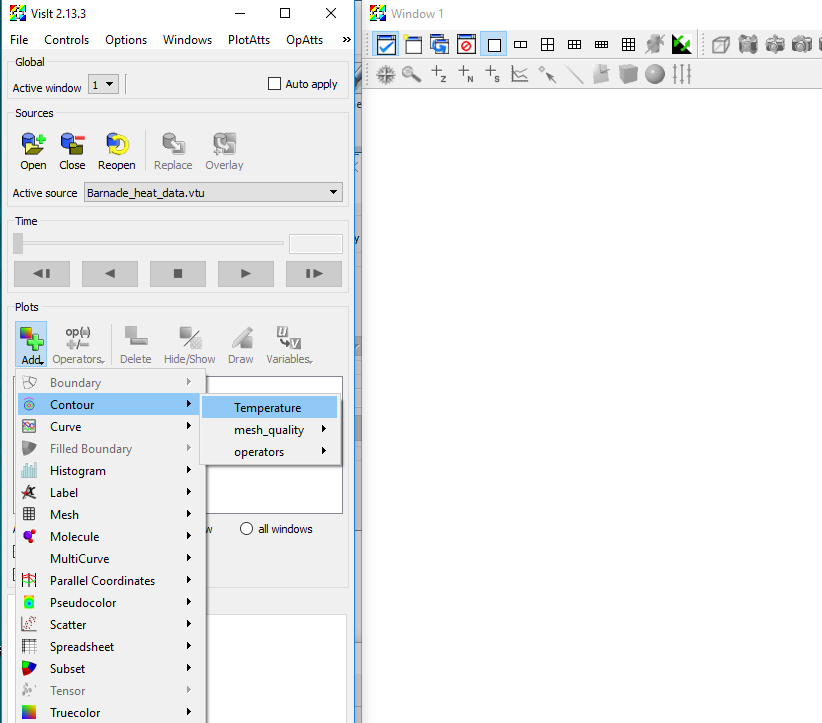
\includegraphics[width=0.6\textwidth]{ch33-comsol-contour.png}\\
\scriptsize \gui{Add $\to$ Contour $\to$ Temperature $\to$ Draw} on it
\end{columns}
\footnotesize
\begin{itemize}
  \item The 2019 ``COMSOL work flow'' lecture solved a heat problem in COMSOL and brought the result into VisIt: in COMSOL, \gui{Results $\to$ Export $\to$ Data}, type \gui{Unstructured *.vtu} (the lecture: ``Export -> Data 1 -> Unstructured *.vtu''; ``not the easiest to find''); in VisIt, \gui{Open} the \code{.vtu} and plot. COMSOL itself is outside this series (chapter 1b lists it); its export is the point here: any program that writes VTK, XML VTK (\code{.vtu}, \code{.vtr}, \code{.vts}), Exodus, Silo, netCDF, HDF5 with a known layout, or plain CSV points can be looked at next to an IBAMR run in the same VisIt window, with the same plots and queries.
\end{itemize}
\sourcecredit{``Lecture 8: COMSOL work flow and remote simulations'' (2019; its COMSOL log is dated 19 February 2019), slides 13--14; the VisIt windows only.}
\end{frame}

% 31
\begin{frame}{ParaView, Tecplot, LCS and circulation: pointers}
\label{fr:others}
\footnotesize
\begin{itemize}
  \item The reverse holds: VisIt's exports (VTK, Silo, Tecplot, STL, PLY, Xmdv) are the way into those programs (slide \ref{fr:export}).
  \item \al{ParaView} (\url{https://www.paraview.org}) opens VTK, XML VTK, Exodus and netCDF natively and, through the VisIt bridge (a ParaView built with it; Silo only when built with the Silo library), SAMRAI dumps and Silo; the lab's 2014 ParaView tutorial PDF and 2021 recording are third-party and listed only. Everything in Part V has a ParaView equivalent (Resample To Image, Slice, Plot Over Line, Python shell); this series chose VisIt because IBAMR's output is written for it.
  \item \al{Tecplot:} the 2017 Read Me notes that Dabiri's LCS code writes ``a data file type for Tecplot'' and that ``Tecplot is like commercial Visit''; VisIt exports Tecplot files (\gui{Export Database $\to$ Tecplot}).
  \item \al{LCS and FTLE:} the 2017 ``LCS options'' slides list VisIt's own \gui{LCS} operator, with FTLE among its outputs (\code{OperatorPlugins()} has \code{LCS}, no separate FTLE), MIT's and ETH's (George Haller's) MATLAB codes; the DabiriLCS Read Me points at Shadden's tutorial and at \code{Convert\_vtk2LCS.m} (slide \ref{fr:vtkm}) for feeding exported fields to it. Chapter 29 runs the VisIt operator.
  \item \al{Circulation:} Arvind's note (2016) lists what his MATLAB script needs from a 2D field, ``x, y, u, v, du/dx, du/dy, dv/dx, dv/dy and z-vorticity''; the note writes the vorticity as $w_z = \partial v/\partial y - \partial u/\partial x$, which is a slip for $\partial v/\partial x - \partial u/\partial y$. The easy version in the same Read Me, ``make a box around the vortex and calculate average vorticity'', is a VisIt query (chapter 29); from a uniform array it is \code{omega[box].mean()}.
  \item \al{The 2017 to-do} that became this chapter: ``Overview of translating one file type to another (.visit, .m, .py, .txt, .vtk, etc)'': the map of slide \ref{fr:map}.
\end{itemize}
\end{frame}

% 32
\begin{frame}{\code{examples/analysis}: the readers, and which chapter uses each}
\label{fr:folder}
\scriptsize
\renewcommand{\arraystretch}{0.95}
\begin{tabular}{@{}L{0.3\textwidth}L{0.46\textwidth}L{0.16\textwidth}@{}}
\toprule
file & what it reads or writes & chapter \\
\midrule
\code{hier\_data.py}, \code{read\_hier\_data.m}, \code{read\_input.m} & the \code{X.*}, \code{F.*} text files; input-file constants & 11 \\
\code{leaf\_forces.py}, \code{leaf\_forces.m} & the drag of IB/03 from the forces (worked example) & 11 \\
\code{samrai\_dumps.py}, \code{samrai\_dumps.m} & the VisIt dumps (HDF5) onto a uniform grid; frames; line fluxes & 33 \\
\code{flow\_rate.py} & the flow rate across lines against time, from the dumps & 33 \\
\code{resample\_export.py} & VisIt CLI: Resample + Export Database over a series of frames & 33, 32 \\
\code{read\_vtk\_legacy.py}, \code{read\_vtk\_legacy.m} & legacy ASCII VTK (VisIt's exports, IB2d's output) & 33 \\
\code{read\_exodus.py}, \code{read\_exodus.m} & the ExodusII file of an IBFE run & 33, 28 \\
\code{hier\_data\_h5.py} & the HDF5 state dumps of the upstream examples & 33 \\
\code{piv\_to\_vtk.py} & two text arrays to a VTK vector field (and any gridded field) & 33, 29 \\
\bottomrule
\end{tabular}

\vspace{1mm}
\footnotesize All Python 3 with \code{numpy}; \code{h5py}, \code{netCDF4} and \code{vtk} where the format needs them (\code{apt install python3-h5py python3-netcdf4 python3-vtk9} on Ubuntu, \code{pip install h5py netCDF4 vtk} elsewhere; VisIt's own Python has none of them, so the VisIt scripts stay inside VisIt and the NumPy scripts outside). The \code{.m} files were checked in Octave 8.4 except \code{samrai\_dumps.m} (no \code{h5read} in Octave).
\end{frame}

% 33
\begin{frame}{Then and now}
\label{fr:thennow}
\scriptsize
\renewcommand{\arraystretch}{0.95}
\begin{tabular}{@{}L{0.44\textwidth}L{0.49\textwidth}@{}}
\toprule
the decks and scripts said (2013--2020) & now \\
\midrule
``Download the matlab-tytell.zip file \ldots run install\_here.m'' (2013) & \code{samrai\_dumps.m} / \code{.py} in \code{examples/analysis}, no toolbox \\
``It is necessary to not output Div U when running IBAMR due to the space in the name'' & not necessary: \code{Div U} is an ordinary HDF5 dataset name \\
\code{V.U\_0}, \code{V.U\_1}, \code{V.F0}, \code{V.F1} (the 2013 field names) & \code{U.00}, \code{U.01} in the files; no \code{F} field in the VisIt dumps of this series' examples (\code{output\_F} off) \\
\code{GridSizex = 4096} typed into the script & read from \code{summary.samrai} (\code{number\_patches}, \code{dx}, \code{ratios}) \\
``record your python commands in visit 2.5.2'' for KillDevil & VisIt 3.5 everywhere, Python 3 inside it (chapter 32) \\
\code{sys.path.append("C:/Program Files/LLNL/VisIt 2.11.0/lib/site-packages")}, \code{frontend.py} edited on Windows & \code{visit -cli} runs the script in VisIt's own Python; no path or hotfix \\
\code{ExportDBAtts.filename = "visit\_ex\_db\_\%s" \% k} & the name is ignored headless in 3.5: rename \code{.vtk} after each export \\
``If you choose no variables, it will just export U'' & true for a plot of \code{U}; add the variables you want, resampled too \\
Nick's reader ``uses only U = (Ux, Uz) in the (x, z) plane'', line numbers built in & \code{read\_vtk\_legacy.m/.py} read the headers; the \code{vtk} module reads anything \\
\code{mopenpiv/vtk\_tools.py} on Bitbucket; \code{toVTK.py} in \code{scripts/forPIV} & both gone; \code{read\_vtk\_legacy.py}, \code{piv\_to\_vtk.py} \\
``Dylan will start overview, Julia will add stuff on techplot'' (the stub) & slide \ref{fr:map} \\
\bottomrule
\end{tabular}
\end{frame}

% 34
\begin{frame}{What can go wrong}
\label{fr:wrong}
\scriptsize
\renewcommand{\arraystretch}{0.95}
\begin{tabular}{@{}L{0.38\textwidth}L{0.55\textwidth}@{}}
\toprule
symptom & cause and fix \\
\midrule
\code{h5py} says ``Unable to open file'' on a \code{lag\_data} file & Silo with the PDB driver: not HDF5; go through VisIt or the \code{X} files \\
the array from a patch looks transposed or scrambled & reshape as \code{(ny, nx)} (x fastest); nodal arrays are one larger per direction \\
the uniform array has NaNs & a level-0 patch missing from the list (a truncated \code{dumps.visit} is not it; a hand-edited summary is); an \code{IndexError} from the ratios table is what you get when \code{uniform} is asked for a level the dump does not have \\
the exported VTK file is empty, or all zeros & one of the traps of slides \ref{fr:empty} and \ref{fr:empty2}: the name, the metadata extents, the zero-thickness slab, the un-resampled multi-patch export, and (in one session) the Vector plot and the magnitude expression \\
\code{meshio.read} fails with \code{'string'} & VisIt's \code{FIELD MeshName} entry; use \code{read\_vtk\_legacy}, the \code{vtk} module or \code{pyvista} \\
\code{ncread} is unknown in Octave & \code{pkg load netcdf} after \code{apt install octave-netcdf} or \code{pkg install -forge netcdf} \\
\code{h5read} is unknown in Octave & there is none in Octave 8; use the Python reader or MATLAB \\
\bottomrule
\end{tabular}
\end{frame}

\begin{frame}{What can go wrong (2)}
\label{fr:wrong2}
\scriptsize
\renewcommand{\arraystretch}{0.95}
\begin{tabular}{@{}L{0.38\textwidth}L{0.55\textwidth}@{}}
\toprule
symptom & cause and fix \\
\midrule
the frames begin at the restart step, the earlier ones missing & \code{dumps.visit} truncated to the frames after the restart: rebuild it (slide \ref{fr:curves}) \\
the flux across one line disagrees with another & the line crosses something besides the channel (a wall, a gap, a second structure), or the AMR level there is coarse: draw the line on the picture first \\
the flow rate differs from the prescribed inflow by a few per cent & the start-up transient; porous point walls; the open box: compare lines with each other first \\
VisIt's Python has no \code{numpy} or \code{h5py} & it is VisIt's own Python: export from VisIt, analyse outside, or install into VisIt's Python at your own risk \\
\bottomrule
\end{tabular}
\end{frame}

% 35
\begin{frame}{Exercises}
\label{fr:exercises}
\footnotesize
\begin{enumerate}
  \item Run \code{samrai\_dumps.py} on a frame of IB/01 and check its \code{Omega} extents against VisIt's \gui{MinMax} query; then plot the uniform array and the patch boxes as on slide \ref{fr:uniform}.
  \item Compute the kinetic energy $\frac12 \rho \int |\mathbf{u}|^2\,dA$ of IB/02's box at every frame from the dumps and plot it against time; compare with the kinetic-energy measure of chapter 9b's pump.
  \item Export the same frame with \code{resample\_export.py} at half the finest spacing and at twice it; read both back and say where they differ from the Python array and why.
  \item Take a plane out of IBFE/10 (\code{viz\_IB3d}) at three heights and plot $U_x$ with \code{read\_vtk\_legacy.py}; then do the same plane with \code{samrai\_dumps.py}'s \code{uniform} and compare the two.
  \item Read IBFE/08's two Exodus files with \code{read\_exodus.py} and compute the gap between the beam's top nodes and the circle's bottom nodes against time (chapter 21's table of the gap at $t = 0, 1, 2, 4$).
  \item Rebuild \code{dumps.visit} of the restart test of chapter 3 and show with \code{sd.frames} that the frames before the restart are back, with their times.
  \item Make a PIV-like field from IB/13's velocity with \code{piv\_to\_vtk.py} at the spacing of a real PIV window ($1$ mm), open it in VisIt next to \code{dumps.visit}, and compare the two with a Pseudocolor of \code{magnitude(U)} and the same limits.
  \item Chapter 24's exercise 6 asks for the average of $T$ from the HDF5 state dump; do it from the VisIt dumps as well (\code{d.uniform("T")}) and check both against chapter 24's table and VisIt's \gui{Average Value} query.
\end{enumerate}
\end{frame}

% 36
\begin{frame}{Rules of thumb}
\label{fr:thumb}
\small
\begin{itemize}
  \item Know the container: HDF5 (dumps, state dumps, netCDF-4 Exodus), Silo PDB (points), text (\code{X}, \code{F}, \code{.curve}); the extension says nothing.
  \item Python for loops over frames and quantities VisIt has no query for; VisIt for pictures and its queries; both give the same numbers.
  \item Nodal arrays are $N + 1$, cell arrays $N$; the files are $x$ fastest; reshape as \code{(ny, nx)}.
  \item Check a reader against the file's own extents and against VisIt once, then trust it.
  \item Headless VisIt exports to \code{<cwd>/.vtk}: rename after every export; give the box yourself.
  \item Rebuild the \code{.visit} lists after a restart before any analysis spans it.
  \item Compare fluxes across two lines before comparing them with anything else.
\end{itemize}
\end{frame}

% 37
\begin{frame}{Summary}
\label{fr:wrapup}
\footnotesize
\begin{enumerate}
  \item An IBAMR run's output is four formats: HDF5 for the fluid dumps (and the upstream examples' state dumps), Silo for the points, netCDF (ExodusII) for finite elements, text for the forces, positions and curves. All but Silo open in Python and MATLAB without VisIt.
  \item \code{samrai\_dumps.py} reads the dumps and assembles the adaptive patches on a uniform grid; VisIt's Resample + Export does the same, and the two agree to single precision.
  \item VTK is the exchange format: VisIt writes it (with five headless traps), IB2d and PIV conversions write it, three readers read it; Exodus and \code{.curve} have readers of their own; the Silo points are the \code{X} files.
  \item The 2013--2020 MATLAB analyses (flow rates, frames with positions) are a loop over frames with the reader; the examples' scripts in \code{examples/analysis} do them on IB/02, IB/11 and IB/13.
  \item Other programs meet IBAMR in VisIt through their VTK or VTU exports; ParaView, Tecplot and the LCS tools take VisIt's exports.
\end{enumerate}
\begin{homebox}
\footnotesize Next: the IB2d chapters (4a--4f), then chapter 27 (3D), 29 (data analysis: queries, lineouts, LCS), 30 (movies), 31 (the cluster) and 32 (the command line and Python, where the recording of slide \ref{fr:script} is taught).
\end{homebox}
\end{frame}

% 38
\begin{frame}{Recordings and screenshots}
\label{fr:videos}
\small
\begin{itemize}
  \item Shannon Jones's YouTube how-tos on recording to Python (\code{watch?v=RASHMJSgYM8}) and on running a script inside VisIt (\code{watch?v=BG7f6rvjHrw}), cited by the 2017--2018 decks and the 2017 Read Me; listed, not incorporated (chapter 32 covers the recording).
  \item The 2021 ParaView tutorial recording (\code{ParaviewTutorial2021.mp4}, third-party) and the COMSOL lecture's recordings are not among the front matter's course recordings; they stay on the Drive.
  \item The window screenshots are the 2017--2018 resampling decks' (VisIt 2.7.1 on a Mac; six of the 2018 deck's images are the 2017 ones), the 2019 PIV document's (DaVis 7.2) and the 2019 COMSOL lecture's two VisIt windows (2.13.3 on Windows); the plot pictures are new (Python and VisIt 3.5 in WSL). The re-shoot list in \code{plan/visit-screenshots-todo.md} has a chapter 33 section (the Resample window, the Export Database window with \gui{Export all time states} and \gui{Add variable}, both in 3.5).
\end{itemize}
\end{frame}

% 39
\begin{frame}{References and credits}
\label{fr:refs}
\scriptsize
\begin{itemize}
  \item The course material: ``Taking a 2D slice from 3D IBAMR with Visit'' (2017) and ``6 -- Resampling AMR grids to Uniform Grid, exporting to .vtk, and recording in Python'' (2018); ``Converting IBAMR output to Matlab and analyzing it'' (MATH 769, 23 April 2013) and ``5 -- Reading forces and converting IBAMR output to Matlab and analyzing it'' (2020); ``6. Analyze PIV Data'' (2019); ``Lecture 8: COMSOL work flow and remote simulations'' (2019); the 2017 lab Read Me notes (``Read Me and To Do'', ``LCS options'', DabiriLCS, circulation, batch processing).
  \item Christopher Strickland, \code{read\_IBAMR3d\_py27.py} and \code{read\_vtk\_data.py} with their README (2017); Nicholas A. Battista, \code{read\_Structured\_Vector\_Field\_Data\_From\_vtk.m} and \code{Convert\_vtk2LCS.m} (2017, \url{http://github.com/nickabattista}); Eric Tytell's \code{importsamrai.m} toolbox (2013; described, not shipped); Lindsay Waldrop's batch-processing note (2017); Julia Samson's OpenPIV instructions (2017); Arvind Santhanakrishnan's circulation note (2016).
  \item SAMRAI's VisIt data writer and HDF5 database: \url{https://computing.llnl.gov/projects/samrai} (\code{VisItDataWriter}, \code{HDFDatabase}); ExodusII: \url{https://sandialabs.github.io/seacas-docs/}; netCDF: \url{https://www.unidata.ucar.edu/software/netcdf/}; the VTK file formats: \url{https://docs.vtk.org/en/latest/design_documents/VTKFileFormats.html}; Silo: \url{https://silo.readthedocs.io/}; h5py, netCDF4-python, meshio, pyvista on PyPI; VisIt's Resample operator and Export Database in the VisIt User Manual.
  \item Data: this series' IB/13, IB/02, IB/11 (\code{FORCE\_VP\_F025}), IBFE/01, IBFE/10 runs and the upstream complex-fluids \code{ex2} run of chapter 25; scripts \code{wsl/final/ch33\_*.sh}, \code{tools/ch33\_figures.py}, \code{tools/ch33\_frames.py}.
\end{itemize}
\end{frame}

\end{document}
